\PassOptionsToPackage{quiet}{xeCJK}
\documentclass[12pt, a4paper, twoside]{ctexbook}
\usepackage{amsmath,amsthm,amssymb,bm,graphicx,hyperref,mathrsfs,geometry,booktabs,makecell,mathcomp,esint,upgreek}
\usepackage{mwe,color,float,cleveref}
\usepackage{tabularx,multirow,array,caption}
\usepackage[T1]{fontenc}

\extrafloats{150}
\graphicspath{{Figures/}}
\hypersetup{colorlinks=true, linkcolor=black}
\geometry{left=2.0cm, top=2.0cm, bottom=2.0cm, right=2.0cm}

\title{{\Huge{\textbf{物理学及其工程应用笔记}}}}
\author{南京工程学院\\Serein}
\date{\today}

\linespread{1.5}
\newCJKfontfamily\sonti{FandolSong-Bold}

\newtheorem{theorem}{定理}[section]
\newtheorem{definition}[theorem]{定义}
\newtheorem{lemma}[theorem]{引理}
\newtheorem{corollary}[theorem]{推论}
\newtheorem{example}[theorem]{例}
\newtheorem{proposition}[theorem]{命题}

\captionsetup{format=hang}
\DeclareCaptionLabelSeparator*{sspace}{\ \ }
\captionsetup[figure]{labelsep=sspace}
\captionsetup[table]{labelsep=sspace}
\DeclareCaptionFont{heiti}{\heiti}
\DeclareCaptionFont{5hao}{\zihao{5}}
\captionsetup{labelfont={heiti,5hao},textfont={heiti,5hao}}

\crefname{figure}{图}{图}
\crefname{table}{表}{表}
\crefname{equation}{式}{式}
\hypersetup{breaklinks,colorlinks}
\hypersetup{hidelinks,bookmarksnumbered=true,bookmarksopen=true,pdfstartview=Fit}

\everymath{\displaystyle}

\begin{document}

\maketitle

% \pagenumbering{roman}
% \setcounter{page}{1}

\newpage
\pagenumbering{Roman} 
\setcounter{page}{1}
\tableofcontents
\newpage
\setcounter{page}{1}
\pagenumbering{arabic}

\chapter{质点运动学与牛顿运动定律}
\newpage
\section{质点运动的描述}
{\sonti 位置矢量}:$\boldsymbol{r}=x\boldsymbol{i}+y\boldsymbol{j}+z\boldsymbol{k}$

{\sonti 运动方程}:$\boldsymbol{r}\left(t\right)=x\left(t\right)\boldsymbol{i}+y\left(t\right)\boldsymbol{j}+z\left(t\right)\boldsymbol{k}$

{\sonti 位移}:$\Delta \boldsymbol{r}$

{\sonti 路程}:$\Delta s$
$$
\Delta s \geqslant \left|\Delta \boldsymbol{r}\right|
$$

{\sonti 平均速度}:
$$
\overline{\boldsymbol{v}}=\frac{\Delta \boldsymbol{r}}{\Delta t}
$$

{\sonti 平均速率}:
$$
\overline{v}=\frac{\Delta s}{\Delta t}
$$

{\sonti 瞬时速度}:
$$
\boldsymbol{v}=\frac{\mathrm{d}\boldsymbol{r}}{\mathrm{d}t}
$$

{\sonti 瞬时速率}:
$$
v=\left|\boldsymbol{v}\right|=\left|\frac{\mathrm{d}\boldsymbol{r}}{\mathrm{d}t}\right|=\frac{\mathrm{d}s}{\mathrm{d}t}=\sqrt{\left(\frac{\mathrm{d}x}{\mathrm{d}t}\right)^2+\left(\frac{\mathrm{d}y}{\mathrm{d}t}\right)^2+\left(\frac{\mathrm{d}z}{\mathrm{d}t}\right)^2}
$$

{\sonti 平均加速度}:
$$
\overline{\boldsymbol{a}}=\frac{\Delta \boldsymbol{v}}{\Delta t}
$$

{\sonti 瞬时加速度}:
$$
\boldsymbol{a}=\frac{\mathrm{d}\boldsymbol{v}}{\mathrm{d}t}= \frac{\mathrm{d}^2\boldsymbol{r}}{\mathrm{d}t^2}
$$
$$
\boldsymbol{a}=a_x\boldsymbol{i}+a_y\boldsymbol{j}+a_z\boldsymbol{k}
$$
$$
a=\sqrt{\left(\frac{\mathrm{d}^2x}{\mathrm{d}t^2}\right)^2+\left(\frac{\mathrm{d}^2y}{\mathrm{d}t^2}\right)^2+\left(\frac{\mathrm{d}^2z}{\mathrm{d}t^2}\right)^2}
$$
\section{曲线运动、圆周运动}
{\sonti 切向}:$\boldsymbol{e}_\tau$

{\sonti 法向}:$\boldsymbol{e}_\mathrm{n}$,这里的$\mathrm{n}$指$\mathrm{normal}$

{\sonti 平均角速度}:
$$
\overline{\boldsymbol{\omega}}=\frac{\Delta \boldsymbol{\theta}}{\Delta t}
$$

{\sonti 瞬时角速度}:
$$
\boldsymbol{\omega}=\frac{\mathrm{d}\boldsymbol{\theta}}{\mathrm{d}t}
$$
角速度方向满足右手定则

{\sonti 平均角加速度}:
$$
\overline{\boldsymbol{\alpha}}=\frac{\Delta\boldsymbol{\omega}}{\Delta t}
$$

{\sonti 角加速度}:
$$
\boldsymbol{\alpha}=\frac{\mathrm{d}\boldsymbol{\omega}}{\mathrm{d}t}= \frac{\mathrm{d}^2\boldsymbol{\theta}}{\mathrm{d}t^2}
$$

{\sonti 角速度与线速度大小关系}:
$$
v=\omega R
$$

{\sonti 切向加速度}:
$$
a_\tau=\frac{\mathrm{d}v}{\mathrm{d}t}=\frac{\mathrm{d}\left(\omega R\right)}{\mathrm{d}t}=\frac{R\mathrm{d}\omega}{\mathrm{d}t}=R\alpha
$$

{\sonti 法向加速度}:
$$
a_\mathrm{n}=\frac{v^2}{\rho}
$$
其中$\rho$为该点曲率半径

特殊地,在圆周运动中,法向加速度为
$$
a_\mathrm{n}=\frac{v^2}{\rho}=\frac{v^2}{R}=w^2R
$$

\section{典型例题}
\begin{example}
    已知某物体在$x$轴上运动,其加速度与位移关系为$a=kx$,初始位置为$x_0$,初速度为$v_0$,试推导该物体运动速度与位移的关系。

    \noindent\textbf{解}

    由$a=kx$,可得
    $$
    \frac{\mathrm{d}v}{\mathrm{d}t}=kx
    $$
    
    因此有
    $$
    \frac{\mathrm{d}v}{\mathrm{d}x}\frac{\mathrm{d}x}{\mathrm{d}t}=kx
    $$
    
    则
    $$
    v\mathrm{d}v=kx\mathrm{d}x
    $$
    
    积分得
    $$
    \int_{v_0}^{v}v\mathrm{d}v=\int_{x_0}^{x}kx\mathrm{d}x
    $$
    
    因此有
    $$
    v^2=v_0^2+k\left(x^2-x_0^2\right)
    $$
\end{example}
\chapter{动量守恒定律与能量守恒定律}
\newpage
\section{基本概念}
{\sonti 线密度}:
$$
\lambda=\frac{m}{l}
$$

{\sonti 面密度}:
$$
\sigma=\frac{m}{S}
$$

{\sonti 体密度}:
$$
\rho=\frac{m}{V}
$$
\section{动量}
{\sonti 动量}是$\boldsymbol{F}$对时间的累积,即
$$
\boldsymbol{I}=\int_{t_1}^{t_2}\boldsymbol{F}\mathrm{d}t=\int_{t_1}^{t_2}m\boldsymbol{a}\mathrm{d}t=m\boldsymbol{v}_2-m\boldsymbol{v}_1=\boldsymbol{p}_2-\boldsymbol{p}_1
$$
$$
\boldsymbol{F}=\frac{\mathrm{d}\boldsymbol{p}}{\mathrm{d}t}
$$

{\sonti 平均冲力}:
$$
\overline{\boldsymbol{F}}\cdot\Delta t=\Delta\boldsymbol{p}
$$

内力不改变系统的动量(作用时间相同),内力可能改变系统的动能,只有外力才可以改变质点系的总动量。动量改变,动能不一定发生改变

动量守恒所列式子中所有速度是相对于地面的
\section{动能}
{\sonti 动能}是$\boldsymbol{F}$对空间的积累,其单位为$\mathrm{J}$,即$\mathrm{N}\cdot\mathrm{m}$

功是标量,表达式为
$$
W=\int\mathrm{d}W=\int_{A}^{B}\boldsymbol{F}\cdot\mathrm{d}\boldsymbol{r}=\int_{A}^{B}F\cos\theta\left|\mathrm{d}\boldsymbol{r}\right|
$$

{\sonti 瞬时功率}:
$$
P=\frac{\mathrm{d}W}{\mathrm{d}t}=\frac{\boldsymbol{F}\cdot\mathrm{d}\boldsymbol{r}}{\mathrm{d}t}=\boldsymbol{F}\cdot\boldsymbol{v}=Fv\cos\theta
$$

{\sonti 平均功率}:
$$
\overline{P}=\frac{W}{t}
$$

功率单位为$\mathrm{W}$

{\sonti 质点的动能定理}:
$$
W=\int_{A}^{B}\boldsymbol{F}\cdot\mathrm{d}\boldsymbol{r}=\frac{1}{2}mv_B^2-\frac{1}{2}mv_A^2=E_{\mathrm{k}B}-E_{\mathrm{k}A}
$$
\section{保守力}
如果力$\boldsymbol{F}$对物体做功只与物体初、末位置有关,而与物体所经历的路程无关,则这种力为\textbf{保守力},否则为\textbf{非保守力}。因此保守力满足的数学表达式为
$$
\oint_l\boldsymbol{F}\cdot\mathrm{d}\boldsymbol{l}=0
$$

重力、弹力、电场力、库伦力、万有引力都属于保守力;摩擦力属于非保守力
\section{势能}
{\sonti 势能表达式}:
\begin{itemize}
    \item 选取无限远点为零势能点,万有引力势能为
    $E_\mathrm{p}=-G\frac{m_1m_2}{r}$
    \item 选取地球表面为零势能点,重力势能为
    $E_\mathrm{p}=mgh$
    \item 选取平衡位置为零势能点,弹簧弹性势能为
    $E_\mathrm{p}=\frac{1}{2}kx^2$
\end{itemize}

势能是属于系统的,其具有相对性,与势能零点有关
\section{功能原理}
{\sonti 质点系的动能定理}:质点系各个质点的合外力功与合内力功之和等于系统动能的增量

{\sonti 质点系的功能原理}:合外力和非保守内力对系统所做的功等于系统机械能的增量

{\sonti 说明}:
\begin{itemize}
    \item 功能原理中,功不含有保守内力的功,有摩擦、阻力做功;而动能定理中含有保守内力的功
    \item 功是能量变化或转化的量度
    \item 能量是系统状态的单值函数
\end{itemize}
\section{机械能守恒定律}
{\sonti 质点系的机械能守恒定律}:当作用于质点系的外力和非保守力不做功或所做功的代数和为零时,质点系的机械能总保持不变
$$
\Delta E_\mathrm{k}=-\Delta E_\mathrm{p}
$$

若题目中提到地球,则说明机械能守恒;若未提及地球,则说明机械能不守恒

机械能=动能+势能
$$
E=E_\mathrm{k}+E_\mathrm{p}
$$
\chapter{连续物体的运动}
\newpage
\section{基本概念}
{\sonti 平均角速度}:
$$
\overline{\boldsymbol{\omega}}=\frac{\Delta \boldsymbol{\theta}}{\Delta t}
$$

{\sonti 角速度}:
$$
\boldsymbol{\omega}=\frac{\mathrm{d}\boldsymbol{\theta}}{\mathrm{d}t}
$$

{\sonti 角加速度}:
$$
\boldsymbol{\alpha}=\frac{\mathrm{d}\boldsymbol{\omega}}{\mathrm{d}t}= \frac{\mathrm{d}^2\boldsymbol{\theta}}{\mathrm{d}t^2}
$$
角速度方向满足右手定则

{\sonti 角速度与线速度大小关系}:
$$
v=\omega R
$$

{\sonti 切向加速度}:
$$
a_\tau=\frac{\mathrm{d}v}{\mathrm{d}t}=\frac{\mathrm{d}\left(\omega R\right)}{\mathrm{d}t}=\frac{R\mathrm{d}\omega}{\mathrm{d}t}=R\alpha
$$

{\sonti 法向加速度}:
$$
a_\mathrm{n}=\frac{v^2}{\rho}
$$
其中$\rho$为该点曲率半径

特殊地,在圆周运动中,法向加速度为
$$
a_\mathrm{n}=\frac{v^2}{\rho}=\frac{v^2}{R}=w^2R
$$
\section{转动定律}
{\sonti 力矩}:
$$
\boldsymbol{M}=\boldsymbol{r}\times\boldsymbol{F}
$$
$$
\left|\boldsymbol{M}\right|=\left|\boldsymbol{r}\right|\left|\boldsymbol{F}\right|\sin\theta=Fd
$$
力矩单位为$\mathrm{N}\cdot\mathrm{m}$,方向满足矢量积的右手定则

{\sonti 注意}:
\begin{figure}[H]
    \centering
    \begin{minipage}{0.48\linewidth}
        \centering
        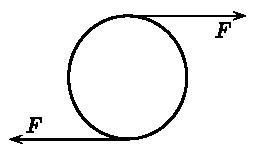
\includegraphics[width=0.6\linewidth]{合外力为零,合外力矩不一定为零.pdf}
        \caption{合外力为零,合外力矩不一定为零}
        \label{fig:合外力为零,合外力矩不一定为零}
    \end{minipage}
    %\qquad
    \begin{minipage}{0.48\linewidth}
        \centering
        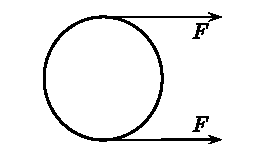
\includegraphics[width=0.6\linewidth]{合外力矩为零,合外力不一定为零.pdf}
        \caption{合外力矩为零,合外力不一定为零}
        \label{fig:合外力矩为零,合外力不一定为零}
    \end{minipage}
\end{figure}
\begin{itemize}
    \item 合外力为零时,合外力矩不一定为零,如\textcolor{blue}{\cref{fig:合外力为零,合外力矩不一定为零}}所示
    \item 合外力矩为零时,合外力不一定为零,如\textcolor{blue}{\cref{fig:合外力矩为零,合外力不一定为零}}所示
\end{itemize}

{\sonti 转动惯量}:用$J$表示,单位为$\mathrm{kg}\cdot\mathrm{m}^2$
\begin{itemize}
    \item $J=\int r^2\mathrm{d}m$:
    \begin{itemize}
        \item 对于长为$l$,质量为$m$的细棒,转轴为其中心,转动惯量为$J=\frac{1}{12}ml^2$
        \begin{figure}[H]
            \centerline{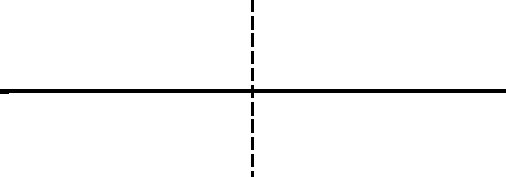
\includegraphics[scale=0.6]{CH03FIG01.pdf}}
        \end{figure}
        由线密度$\lambda=\frac{m}{l}$,有
        $$
        \mathrm{d}\left(\lambda r\right)=\mathrm{d}m \Rightarrow \lambda\mathrm{d}r=\mathrm{d}m \Rightarrow \frac{m}{l}\mathrm{d}r=\mathrm{d}m
        $$
        因此
        $$
        J=\int r^2 \mathrm{d}m=\frac{m}{l}\int_{-\frac{l}{2}}^{\frac{l}{2}} r^2 \mathrm{d}r=\frac{1}{12}ml^2
        $$

        \item 对于长为$l$,质量为$m$的细棒,转轴为其边端,转动惯量为$J=\frac{1}{3}ml^2$
        \begin{figure}[H]
            \centerline{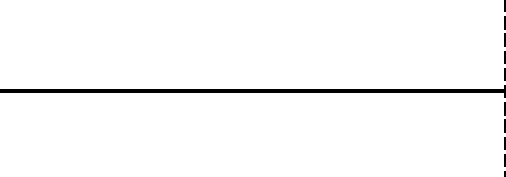
\includegraphics[scale=0.6]{CH03FIG02.pdf}}
        \end{figure}
        $$
        J=\int r^2 \mathrm{d}m=\frac{m}{l}\int_{0}^{l} r^2 \mathrm{d}r=\frac{1}{3}ml^2
        $$
        \item 对于半径为$R$,质量为$m$的圆环,转轴为其中心,转动惯量为$J=mR^2$
        \begin{figure}[H]
            \centerline{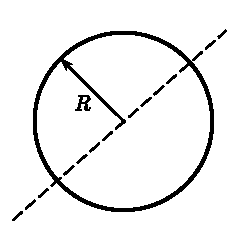
\includegraphics[scale=1.0]{CH03FIG03.pdf}}
        \end{figure}
        $$
        J=\int R^2 \mathrm{d}m=mR^2
        $$
        \item 对于半径为$R$,质量为$m$的薄圆盘,转轴为其中心,转动惯量为$J=\frac{1}{2}mR^2$
        \begin{figure}[H]
            \centerline{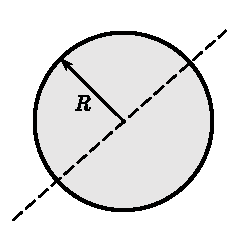
\includegraphics[scale=1.0]{CH03FIG04.pdf}}
        \end{figure}
        由面密度$\sigma=\frac{m}{S}$,有
        $$
        \mathrm{d}\left(\sigma s\right)=\mathrm{d}m \Rightarrow \sigma\mathrm{d}\left(\pi r^2\right)=\mathrm{d}m \Rightarrow \frac{m}{S}\cdot2\pi r\mathrm{d}r=\mathrm{d}m
        $$
        因此
        $$
        J=\int r^2\mathrm{d}m=\frac{2\pi m}{\pi R^2}\int_{0}^{R} r^3\mathrm{d}r=\frac{1}{2}mR^2
        $$
        \item 质点:$J=\sum_{i=1}^{n}m_ir_i^2$
    \end{itemize}
\end{itemize}

转动惯量$J$(对于某一转轴而言)与质量、质量分布、转轴位置有关
$$
M=J\alpha
$$
$$
M=rF\sin\theta=rF_\tau=rma_\tau=rmr\alpha=\alpha mr^2=J\alpha
$$

{\sonti 平行轴定理}:质量为$m$的刚体对过它质心的轴$zC$的转动惯量为$J_C$,若有另一轴线$zO$与$zC$平行,两轴之间的距离为$d$,如\textcolor{blue}{\cref{fig:平行轴定理}}所示
\begin{figure}[H]
    \centerline{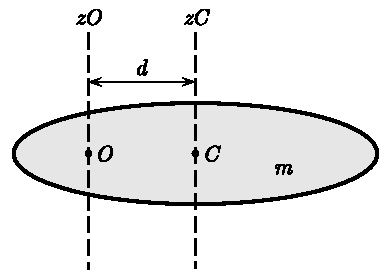
\includegraphics[scale=1.2]{平行轴定理.pdf}}
    \caption{平行轴定理}\label{fig:平行轴定理}
\end{figure}
\noindent{则刚体对$zO$轴的转动惯量为}
$$
J_O=J_C+md^2
$$

\begin{example}
    一质量为$m$、长为$l$的匀质细杆,与质量为$m$、半径为$R$的小球相连。求它们相对于过$O$点水平轴的转动惯量。
    \begin{figure}[H]
        \centerline{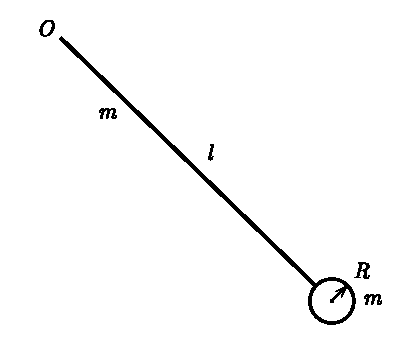
\includegraphics[scale=0.8]{CH03EX01.pdf}}
    \end{figure}
    \noindent\textbf{解}

    $l$,$m$对$O$
    $$
    J_1=\frac{1}{3}ml^2
    $$

    $R$,$m$对$O$
    $$
    J_2=J_{\text{球}}+m\left(l+R\right)^2=\frac{2}{5}mR^2+m\left(l+R\right)^2
    $$

    因此
    $$
    J=J_1+J_2=\frac{1}{3}ml^2+\frac{2}{5}mR^2+m\left(l+R\right)^2=\frac{4}{3}ml^2+\frac{7}{5}mR^2+2mRl
    $$
\end{example}
\begin{example}
    质量为$m_3$,半径为$R$的定滑轮(可视为质量均匀分布的圆盘),一根轻绳跨过定滑轮(轻绳不能伸长,绳与定滑轮之间无相对滑动,忽略定滑轮轴处的摩擦),绳的两端分别悬挂质量为$m_1$,$m_2$的物块,且$m_2>m_1$。求物块运动的加速度和轻绳的张力。
    \begin{figure}[H]
        \centerline{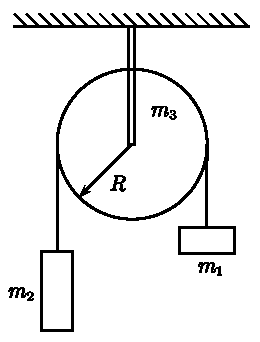
\includegraphics[scale=0.8]{CH03EX02.pdf}}
    \end{figure}
    \noindent\textbf{解}
    $$
    \left\{ \begin{array}{l}
        m_2g-T_2=m_2a\\
        T_1-m_1g=m_1a\\
        T_2R-T_1R=J\alpha\\
        J=\frac{1}{2}m_3R^2\\
        a=R\alpha\\
    \end{array} \right. \Rightarrow 
    \left\{ \begin{array}{l}
        a=\frac{\left( m_2-m_1 \right) g}{m_1+m_2+\frac{1}{2}m_3}\\
        T_1=\frac{m_1\left( 2m_2+\frac{1}{2}m_3 \right) g}{m_1+m_2+\frac{1}{2}m_3}\\
        T_2=\frac{m_2\left( 2m_1+\frac{1}{2}m_3 \right) g}{m_1+m_2+\frac{1}{2}m_3}\\
    \end{array} \right. 
    $$
\end{example}
\section{角动量}
{\sonti 质点的角动量}:
$$
\boldsymbol{L}=\boldsymbol{r}\times\boldsymbol{p}
$$
角动量大小为
$$
L=rmv=rm\omega r=\omega mr^2=J\omega
$$

{\sonti 质点的角动量定理}:
$$
\boldsymbol{M}=\frac{\mathrm{d}\boldsymbol{L}}{\mathrm{d}t}
$$
$$
\int_{t_1}^{t_2}\boldsymbol{M}\mathrm{d}t=\boldsymbol{L}_2-\boldsymbol{L}_1
$$

{\sonti 质点的角动量守恒定律}:

合外力矩为零时,即$\boldsymbol{M}=0$,则$\boldsymbol{L}$为常矢量

角动量守恒,合外力矩为零

内力矩不改变系统的角动量

{\sonti 刚体定轴转动的角动量}:
$$
\boldsymbol{L}=J\boldsymbol{\omega}
$$

{\sonti 刚体定轴转动的角动量定理}:
$$
\int_{t_1}^{t_2}M\mathrm{d}t=\int_{L_1}^{L_2}\mathrm{d}L=L_2-L_1
$$

当转动惯量一定时,有
$$
\int_{t_1}^{t_2}M\mathrm{d}t=J\omega_2-J\omega_1
$$

当转动惯量变化时,有
$$
\int_{t_1}^{t_2}M\mathrm{d}t=J_2\omega_2-J_1\omega_1
$$
\begin{example}
    一均匀细杆长为$l$,质量为$m$,平放在摩擦因数为$\mu$的水平桌面上,设开始时杆以角速度$\omega_0$绕过中心$O$且垂直于桌面的轴转动。求作用于杆的摩擦力矩以及杆停止转动所经历的时间。
    \begin{figure}[H]
        \centerline{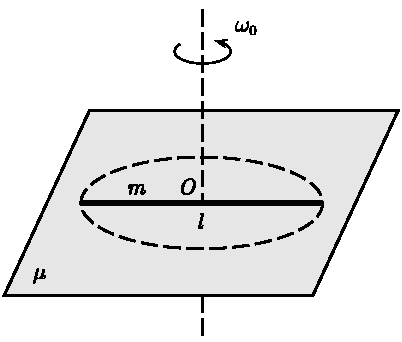
\includegraphics[scale=1.0]{CH03EX03.pdf}}
    \end{figure}
    \noindent\textbf{解}

    {\sonti 作用于杆的摩擦力矩}:

    由线密度$\lambda=\frac{m}{l}$,有
    $$
    \frac{m}{l}\mathrm{d}r=\mathrm{d}m
    $$
    
    因此
    $$
    \mathrm{d}f=\mu\left(\mathrm{d}m\right)g=\frac{\mu mg}{l}\mathrm{d}r
    $$
    $$
    \mathrm{d}M=r\mathrm{d}f=\frac{\mu mg}{l}r\mathrm{d}r
    $$
    
    所以
    $$
    M=2\int_{0}^{\frac{l}{2}}\frac{\mu mg}{l}r\mathrm{d}r=\frac{1}{4}\mu mgl
    $$

    {\sonti 杆停止转动所经历的时间}:
    $$
    M=J\alpha=J\frac{\mathrm{d}\omega}{\mathrm{d}t}
    $$

    因此
    $$
    M\mathrm{d}t=J\mathrm{d}\omega
    $$

    从而有
    $$
    \int_{0}^{t}\left(-M\right)\mathrm{d}t=\int_{\omega_0}^{0}J\mathrm{d}\omega
    $$

    且
    $$
    J=\frac{1}{12}ml^2
    $$

    因此
    $$
    -\frac{1}{4}\mu mglt=-\frac{1}{12}ml^2\omega_0
    $$

    得
    $$
    t=\frac{\omega_0l}{3\mu g}
    $$

    \noindent\textbf{另解}

    根据刚体的角动量定理
    $$
    -Mt=J\omega-J\omega_0
    $$

    代入
    $$
    \left\{ \begin{array}{l}
	    J=\frac{1}{12}ml^2   \\
	    \omega =0  \\
	    M=\frac{1}{4}\mu mgl    \\
    \end{array} \right. 
    $$

    得
    $$
    t=\frac{\omega_0l}{3\mu g}
    $$

    因此杆经过$t=\frac{\omega_0l}{3\mu g}$才会停止转动
\end{example}
{\sonti 刚体定轴转动的角动量守恒定律}:当刚体所受的合外力矩为零,或者不受合外力的作用,刚体的角动量保持不变
$$
\boldsymbol{M}=0 \Rightarrow J\boldsymbol{\omega}=\text{常矢量}
$$
$$
J\omega=J_0\omega_0
$$

{\sonti 平动与转动的动能与动能定理}:
\begin{itemize}
    \item {\sonti 动能}:
    \begin{itemize}
        \item 平动:$\frac{1}{2}mv^2$
        \item 转动:$\frac{1}{2}J\omega^2$
    \end{itemize}
    \item {\sonti 动能定理}:
    \begin{itemize}
        \item 平动:$W=\frac{1}{2}mv_2^2-\frac{1}{2}mv_1^2$
        \item 转动:$W=\frac{1}{2}J\omega_2^2-\frac{1}{2}J\omega_1^2$
    \end{itemize}
\end{itemize}
\section{力矩的功与功率}
{\sonti 力矩的功}:合外力矩所做的元功等于力矩与角位移的乘积
$$
W=\int M\mathrm{d}\theta
$$

{\sonti 力矩的功率}:
$$
P=\frac{\mathrm{d}W}{\mathrm{d}t}=\frac{M\mathrm{d}\theta}{\mathrm{d}t}=M\omega
$$
\section{刚体定轴转动的动能定理}
合外力矩对绕定轴转动的刚体所做的功,等于刚体的转动动能的增量
$$
M=J\alpha=J\frac{\mathrm{d}\omega}{\mathrm{d}t} \Rightarrow W=\int J\frac{\mathrm{d}\omega}{\mathrm{d}t}\mathrm{d}\theta=\int_{\omega_1}^{\omega_2} J\omega\mathrm{d}\omega=\frac{1}{2}J\omega_2^2-\frac{1}{2}J\omega_1^2
$$

{\sonti 势能的变化}:
$$
\Delta E_{\mathrm{p}}=mg\Delta h_{\mathrm{c}}
$$
其中$\Delta h_{\mathrm{c}}$为物体质心高度的变化
\newpage
\section{角动量守恒}
\begin{itemize}
    \item {\sonti 子弹打棒}:设质量为$m$的子弹以速度$v$射入质量为$m'$,长度为$l$的木棒
    \begin{itemize}
        \item \textbf{子弹射入木棒底端}:
        \begin{figure}[H]
            \centerline{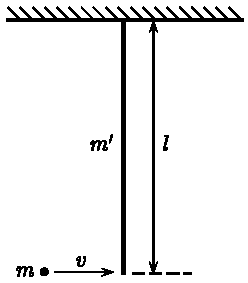
\includegraphics[scale=0.88]{子弹打木块A.pdf}}
        \end{figure}
        \begin{itemize}
            \item 子弹打入木棒,有
            $$
            lmv=\left[ml^2+\frac{1}{3}m'l^2\right]\omega
            $$
            \item 子弹从木棒中射出,射出速度为$v_1$,有
            $$
            lmv=\frac{1}{3}m'l^2\omega+lmv_1
            $$
            \item 子弹被木棒反弹,子弹反弹的速度为$v_2$,方向与初速度方向相反,有
            $$
            lmv=\frac{1}{3}m'l^2\omega-lmv_2
            $$
        \end{itemize}
        \item \textbf{子弹射入木棒某一位置,距木棒顶端距离为}$a$:
        \begin{figure}[H]
            \centerline{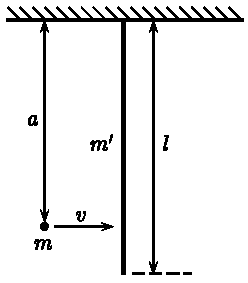
\includegraphics[scale=0.88]{子弹打木块B.pdf}}
        \end{figure}
        \begin{itemize}
            \item 子弹打入木棒,有
            $$
            amv=\left[ma^2+\frac{1}{3}m'l^2\right]\omega
            $$
            \item 子弹从木棒中射出,射出速度为$v_1$,有
            $$
            amv=\frac{1}{3}m'l^2\omega+amv_1
            $$
            \item 子弹被木棒反弹,子弹反弹的速度为$v_2$,方向与初速度方向相反,有
            $$
            amv=\frac{1}{3}m'l^2\omega-amv_2
            $$
        \end{itemize} 
    \end{itemize}
    \item {\sonti 运动员}:
    $$
    J\omega=J_0\omega_0
    $$
    \item {\sonti 天体运动}:
    $$
    R_1mv_1=R_2mv_2
    $$
    \item {\sonti 盘}:
    $$
    J\omega=0+\left(J+mR^2\right)\omega
    $$
\end{itemize}
\section{碰撞}
{\sonti 完全弹性碰撞}:动量守恒+动能守恒

{\sonti 完全非弹性碰撞}:动量守恒(有能量损失)

{\sonti 有刚体参与的碰撞}:通常利用系统角动量守恒求解
\begin{example}
    质量为$m$,长度为$2l$的均匀细棒,静止放置在光滑的水平面上,可以绕通过其中心的转轴转动。质量为$m_2$的小球以速度$v_0$垂直撞到棒的端点并反向弹回。设小球与棒作完全弹性碰撞,求碰撞后,小球的速度和棒的角速度。
    
    \noindent\textbf{解}
    $$
    \left\{ \begin{array}{l}
	m_2v_0l=-m_2vl+J\omega\\
	\frac{1}{2}m_2v_{0}^{2}=\frac{1}{2}m_2v^2+\frac{1}{2}J\omega ^2\\
	J=\frac{1}{12}m\left( 2l \right) ^2\\
    \end{array}\Rightarrow \left\{ \begin{array}{l}
	v=\frac{m_1-3m_2}{m_1+3m_2}v_0\\
	\omega =\frac{6m_2}{\left( m_1+3m_2 \right) l}v_0\\
    \end{array} \right. \right. 
    $$
\end{example}
\section{流体力学}
{\sonti 理想流体的连续性方程}:
$$
Sv=\mathrm{const}
$$

{\sonti 伯努利方程}:
$$
p+\frac{1}{2}\rho v^2+\rho gy=\mathrm{const}
$$
\chapter{机械振动}
\newpage
\section{简谐振动}
{\sonti 简谐振动的微分方程}:
$$
\frac{\mathrm{d}^2x}{\mathrm{d}t^2}+\omega^2 x=0
$$

{\sonti 简谐振动的微分方程解的表示}:
$$
x=A\cos\left(\omega t+\varphi\right)
$$

令$t=0$,则$x_0=A\cos\varphi$

{\sonti 速度}:
$$
v=\frac{\mathrm{d}x}{\mathrm{d}t}=-A\omega\sin\left(\omega t+\varphi\right)
$$

令$t=0$,可得初速度$v_0=-A\omega\sin\varphi$。

速度最大值为$v_{\max}=A\omega$

{\sonti 加速度}:
$$
a=\frac{\mathrm{d}v}{\mathrm{d}t}=\frac{\mathrm{d}^2x}{\mathrm{d}t^2}=-A\omega^2\cos\left(\omega t+\varphi\right)
$$

加速度最大值为$a_{\max}=A\omega^2$

由
$$
\left\{ \begin{array}{l}
	x_0=A\cos \varphi\\
	v_0=-A\omega \sin \varphi\\
\end{array} \right. \Rightarrow \left\{ \begin{array}{l}
	wx_0=A\omega \cos \varphi\\
	v_0=-A\omega \sin \varphi\\
\end{array} \right. 
$$

可得
$$
\omega^2x_0^2+v_0^2=A^2\omega^2
$$
$$
\frac{-A\omega\sin\varphi}{A\cos\varphi}=\frac{v_0}{x_0}
$$

因此
$$
A^2=x_0^2+\frac{v_0^2}{\omega^2}
$$

从而
$$
A=\sqrt{x_0^2+\left(\frac{v_0}{\omega}\right)^2}
$$
$$
\tan\varphi=-\frac{v_0}{x_0\omega}
$$

{\sonti 弹簧振子}:
$$
\boldsymbol{F}=-k\boldsymbol{x}
$$
$$
\omega^2=\frac{k}{m} \Rightarrow \omega=\sqrt{\frac{k}{m}}
$$
$$
\left\{ \begin{array}{l}
	T=\frac{2\pi}{\omega}=2\pi \sqrt{\frac{m}{k}}\\
	\nu =\frac{1}{T}=\frac{\omega}{2\pi}=\frac{1}{2\pi}\sqrt{\frac{k}{m}}\\
\end{array} \right. 
$$
\newpage
{\sonti 描述简谐振动的几个特征量}:
\begin{itemize}
    \item 幅度$A$,$\mathrm{m}$:$A=\sqrt{x_0^2+\left(\frac{v_0}{\omega}\right)}$
    \item 周期$T$,$\mathrm{s}$:$T=\frac{2\pi}{\omega}$
    \item 频率$\nu$,$\mathrm{Hz}$:$\nu=\frac{1}{T}=\frac{\omega}{2\pi}$
    \item 角频率$\omega$,$\mathrm{rad}\cdot\mathrm{s}^{-1}$:$\omega=2\pi\nu=\frac{2\pi}{T}$
    \item 相位:$\omega t+\varphi$,当$t=0$时,可得初相位为$\varphi$
\end{itemize}

{\sonti 几个关于周期的和结论}:
\begin{itemize}
    \item 弹簧振子:
    $$
    T=2\pi\sqrt{\frac{m}{k}}
    $$
    当弹簧振子串联时,有
    $$
    \frac{1}{k}=\frac{1}{k_1}+\frac{1}{k_2}+\cdots+\frac{1}{k_n}
    $$
    当弹簧振子并联时,有
    $$
    k=k_1+k_2+\cdots+k_n
    $$
    \item 单摆:
    $$
    T=2\pi\sqrt{\frac{l}{g}}
    $$
    \item 复摆:
    $$
    T=2\pi\sqrt{\frac{J}{mgl}}
    $$
    其中$J$为绕转轴的转动惯量,$l$为质心到转轴的距离
\end{itemize}
\section{旋转矢量法}
画出矢量圆,矢量端点$P$在$x$轴上的投影点作简谐运动,当圆上某一点在\uppercase\expandafter{\romannumeral1},\uppercase\expandafter{\romannumeral2}象限时,该点速度$v<0$;当圆上某一点在\uppercase\expandafter{\romannumeral3},\uppercase\expandafter{\romannumeral4}象限时,该点速度$v>0$

{\sonti 旋转矢量法的应用}:
\begin{itemize}
    \item 求初相位$\varphi$:绘制出矢量圆,依据$y-t$图像$x=0$处的斜率,得到该点$v$与$0$的关系,并依据该点位置,在矢量圆标出,即可求得初相位$\varphi$
    \item 求$\omega$:
    $$
    \Delta\varphi=\omega\Delta t
    $$
    \item 求最短时间:
    $$
    \Delta\varphi=\omega\Delta t
    $$
    $$
    \frac{2\pi}{T}\Delta t=\Delta\varphi
    $$
\end{itemize}
\section{简谐振动的能力}
{\sonti 弹簧振子的弹性势能}:
$$
E_{\mathrm{p}}=\frac{1}{2}kx^2=\frac{1}{2}kA^2\cos^2\left(\omega t+\varphi\right)=\frac{1}{2}m\omega^2A^2\cos^2\left(\omega t+\varphi\right)
$$

{\sonti 弹簧振子的动能}:
$$
E_{\mathrm{k}}=\frac{1}{2}mv^2=\frac{1}{2}m\omega A^2\sin^2\left(\omega t+\varphi\right)
$$

{\sonti 弹簧振子的机械能}:
$$
E=E_{\mathrm{p}}+E_{\mathrm{k}}=\frac{1}{2}m\omega^2A^2=\frac{1}{2}kA^2
$$
$$
\omega^2=\frac{k}{m}
$$

位移最大,势能最大,动能为零,$a$有最大值

平衡位置,势能为零,动能最大,$v$有最大值
$$
T_\mathrm{k,p}=\frac{1}{2}T_\text{振}
$$
$$
f_\mathrm{k,p}=2f_\text{振}
$$
\section{简谐振动的合成}
{\sonti 同方向同频率简谐振动的合成}:

记两列波的振动方程为
$$
x_1=A_1\cos\left(\omega t+\varphi_1\right)
$$
$$
x_2=A_2\cos\left(\omega t+\varphi_2\right)
$$

则合成的振动方程为
$$
x=x_1+x_2
$$
\begin{figure}[H]
    \centerline{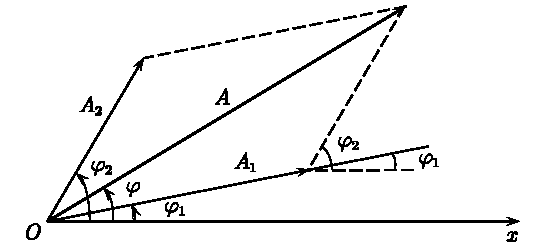
\includegraphics[scale=0.88]{同方向同频率简谐振动的合成.pdf}}
    \caption{同方向同频率简谐振动的合成}\label{fig:同方向同频率简谐振动的合成}
\end{figure}
如\textcolor{blue}{\cref{fig:同方向同频率简谐振动的合成}}所示,由余弦定理,可以得到
$$
\cos\left[\pi-\left(\varphi_2-\varphi_1\right)\right]=\frac{A_1^2+A_2^2-A^2}{2A_1A_2}
$$

因此
$$
A=\sqrt{A_1^2+A_2^2+2A_1A_2\cos\left(\varphi_2-\varphi_1\right)}
$$

不妨记$\Delta\varphi=\varphi_2-\varphi_1$,则
\begin{itemize}
    \item 当$\Delta\varphi=\varphi_2-\varphi_1=\pm 2k\pi$时,合振幅最大,振动加强,$A=A_1+A_2$
    \item 当$\Delta\varphi=\varphi_2-\varphi_1=\pm\left(2k+1\right)\pi$时,合振幅最小,振动减弱,$A=\left|A_1-A_2\right|$,$\varphi=\max\left\{\varphi_1,\varphi_2\right\}$
    \item 当$\Delta\varphi=\varphi_2-\varphi_1$取其他值时,有$\left|A_1-A_2\right|<A<A_1+A_2$
\end{itemize}

{\sonti 同方向不同频率简谐振动的合成}:

拍振幅从极大到下一次极大,中间经历的时间$T$称为周期,显然
$$
T=\frac{2\pi}{\omega_2-\omega_1}
$$

单位时间内拍振幅大小变化的次数称为拍频,即
$$
\nu=\frac{\omega_2-\omega_1}{2\pi}=\nu_2-\nu_1
$$
\chapter{机械波}
\newpage
\section{基本概念}
{\sonti 波动方程}:$y\left(x,t\right)$
\begin{itemize}
    \item $x$为各点振动时平衡位置的坐标
    \item $y$为离开平衡位置的位移
\end{itemize}

{\sonti 机械波}的产生需要\textbf{波源}及\textbf{介质}

{\sonti 振动与波动}:
\begin{itemize}
    \item 振动:波形成的原因,$y-t$
    \item 波动:振动状态的传播,$y-x$
\end{itemize}

{\sonti 描述波动过程的几个特征量}:
\begin{itemize}
    \item 波长$\lambda$,$\mathrm{m}$:$\lambda=Tu=\frac{u}{v}$
    \item 周期$T$,$\mathrm{s}$:$T=\frac{1}{\nu}=\frac{\lambda}{u}$
    \item 波速$u$,$\mathrm{m}\cdot\mathrm{s}^{-1}$:$u=\frac{\lambda}{T}=\lambda\nu$
    \item 频率$\nu$,$\mathrm{Hz}$:$\nu=\frac{1}{T}$
\end{itemize}

周期与频率只决定于波源的振动;波速只决定于介质的性质,与振源无关

\textbf{在均匀各向同性固体介质中}:
\begin{itemize}
    \item {\sonti 纵波波速}:
    $$
    u=\sqrt{\frac{E}{\rho}}
    $$
    其中$E$为介质的弹性模量,$\rho$为介质的密度
    \item {\sonti 横波波速}:
    $$
    u=\sqrt{\frac{G}{\rho}}
    $$
    其中$G$为介质的切变模量
\end{itemize}

\textbf{在液体和气体中}:
\begin{itemize}
    \item {\sonti 纵波波速}:
    $$
    u=\sqrt{\frac{K}{\rho}}
    $$
    其中$K$为体积模量
\end{itemize}

\textbf{横波不能在液体和气体中传播}

{\sonti 波线、波面、波前}:
\begin{itemize}
    \item {\sonti 波线}:沿波的传播方向作一些带箭头的线
    \item {\sonti 波面}:某时刻介质中各振动相位相同的点联结成的面
    \item {\sonti 波前}:位于最前面的领先波面
\end{itemize}

同一波阵面上各点振动状态相同,波线恒与波面垂直
\section{平面简谐波的波函数}
平面简谐波的波函数即为波动方程
\begin{itemize}
    \item 波沿$x$轴正方向传播,平面简谐波的波函数为
    $$
    y=A\cos\left[\omega\left(t-\frac{x}{u}\right)+\varphi\right]
    $$
    \item 波沿$y$轴负方向传播,平面简谐波的波函数为
    $$
    y=A\cos\left[\omega\left(t+\frac{x}{u}\right)+\varphi\right]
    $$
\end{itemize}
$$
\omega=\frac{2\pi}{T}=2\pi\nu
$$
$$
u=\frac{\lambda}{T}=\lambda\nu
$$
$$
\frac{\omega}{u}=\frac{2\pi\nu}{\lambda\nu}=\frac{2\pi}{\lambda}
$$
\begin{itemize}
    \item {\sonti 振动方程}:描述某一质点在任意时刻偏离平衡位置的位移,$y=f\left(t\right)$
    \item {\sonti 波动方程}:描述任意一个质点在任意时刻偏离平衡位置的位移,$y=f\left(x,t\right)$
\end{itemize}
\begin{example}
    某简谐振动的波动方程在$t=0$时刻图像如下图所示,其沿$x$轴正方向传播,且在$x=0$处,$y=-\frac{A}{2}$,求波动的初相位。
    \begin{figure}[H]
        \centerline{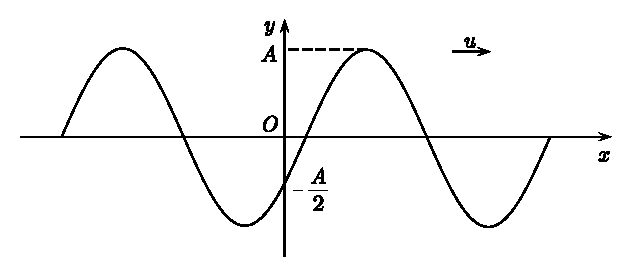
\includegraphics[width=0.5\textwidth]{CH04EX01.pdf}}
    \end{figure}

    \noindent\textbf{解}

    由图像,在$t=0$时刻,$x=0$处,可得$v<0$
    \begin{figure}[H]
        \centering
        \begin{minipage}{0.50\linewidth}
            \centering
            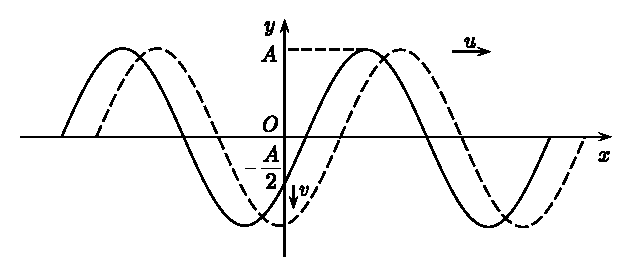
\includegraphics[width=1.0\linewidth]{CH04EX01SolveA.pdf}
        \end{minipage}
        \begin{minipage}{0.48\linewidth}
            \centering
            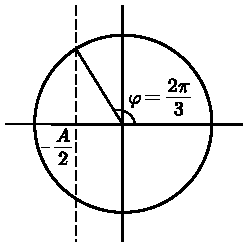
\includegraphics[width=0.44\linewidth]{CH04EX01SolveB.pdf}
        \end{minipage}
    \end{figure}
    再由旋转矢量法,可得$\varphi=\frac{2\pi}{3}$
\end{example}

{\sonti 以沿$x$轴正方向传播的波为研究对象}:
$$
y=A\cos\left[\omega\left(t-\frac{x}{u}\right)+\varphi\right]
$$
$$
u=\frac{\partial y}{\partial t}=-A\omega\sin\left[\omega\left(t-\frac{x}{u}\right)+\varphi\right]
$$
$$
a=\frac{\partial^2 y}{\partial t^2}=\frac{\partial u}{\partial t}=-A\omega^2\cos\left[\omega\left(t-\frac{x}{u}\right)+\varphi\right]
$$

{\sonti 相位差}:
$$
\Delta\varphi=\frac{2\pi}{\lambda}\Delta x=\frac{2\pi}{\lambda}\Delta
$$
$$
\Delta\varphi=\omega\Delta t
$$
\section{波的能量}
体积元机械能不守恒,但平均能量密度不变,为
$$
\overline{w}=\frac{1}{2}\rho A^2 \omega^2
$$
这说明介质中无能量的累积

体积元的动能=体积元的势能

\begin{itemize}
    \item 在平衡位置时,体积元的动能、势能、总机械能均最大
    \item 在最大位移处时,体积元的动能、势能、总机械能均最小,为零
\end{itemize}

{\sonti 能流}:
$$
p=wuS
$$
其中$w$为单位体积中波的能量,$S$为均匀介质垂直于波速$u$的面积

{\sonti 平均能流}:
$$
\overline{p}=\overline{w}uS
$$

{\sonti 能流密度}:
$$
I=\frac{\overline{p}}{S}=\overline{w}u=\frac{1}{2}\rho A^2 \omega^2 u
$$
其中$\rho$为介质密度,$A$为波的振幅,$\omega$为角频率,$u$为波速

\section{波的衍射与干涉}
{\sonti 明显衍射条件}:障碍物尺寸可与波长相比,甚至比波长更小

{\sonti 波的衍射}:波在传播中遇到障碍物,其传播方向发生改变,并可绕过障碍物而继续向前传播

{\sonti 波的干涉}:两列频率相同、振动方向相同、相位差恒定的简谐波叠加,空间某些点处的振动始终加强,另一些点处振动始终减弱,呈现规律性分布。能产生干涉现象的波称为相干波,相应的波源称为相干波源
$$
A=\sqrt{A_1^2+A_2^2+2A_1A_2\cos\left(\varphi_2-\varphi_1-2\pi\cdot\frac{r_2-r_1}{\lambda}\right)}
$$

不妨令$\Delta\varphi=\varphi_2-\varphi_1-2\pi\cdot\frac{r_2-r_1}{\lambda}$
\begin{itemize}
    \item 当$\Delta\varphi=2k\pi$时,振动加强,$A=A_1+A_2$
    \item 当$\Delta\varphi=\left(2k+1\right)\pi$时,振动减弱,$A=\left|A_1-A_2\right|$
\end{itemize}

记$\delta=r_2-r_1$为波程差,若当两列波初相位相同时,即$\varphi_1=\varphi_2$,则
\begin{itemize}
    \item 当$\delta=\pm k\lambda$(即半波长的偶数倍)时,振动加强
    \item 当$\delta=\pm \left(2k-1\right)\lambda$(即半波长的奇数倍)时,振动减弱
\end{itemize}
\section{驻波}
若让两列振幅相同,传播方向相反的相干波叠加,在一定条件下可以形成驻波,驻波是干涉的特例,驻波表达式为
$$
y=\left[2A\cos\left(\frac{2\pi}{\lambda}x\right)\right]\cos\left(\omega t\right)
$$
其中$\left[2A\cos\left(\frac{2\pi}{\lambda}x\right)\right]$为简谐振动的振幅

驻波波形如\textcolor{blue}{\cref{fig:驻波波形}}所示
\begin{figure}[H]
    \centerline{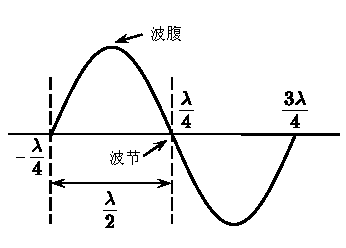
\includegraphics[scale=1.14]{驻波波形.pdf}}
    \caption{驻波波形}\label{fig:驻波波形}
\end{figure}

\begin{itemize}
    \item 波节:$x=\pm\left(2k+1\right)\cdot\frac{\lambda}{4}$,振幅为零处
    \item 波腹:$x=\pm\frac{k}{2}\lambda$,振幅最大处
\end{itemize}

相邻波节之间的距离为$\frac{\lambda}{2}$,相邻波腹之间的距离也为$\frac{\lambda}{2}$

相邻波节之间,相位相同,振幅不全相等;波节两侧,相位相反

驻波不能传播能量,驻波波节处始终不动,动能主要集中在波腹,势能主要集中在波节

在自由端反射时无半波损失,在固定端反射时有半波损失

波从波疏介质入射到波密介质,反射时存在半波损失,从波密介质入射到波疏介质,反射时无半波损失

当波从波疏介质入射到波密介质,被反射回波疏介质时,在反射处形成波节,相位有$\pi$的突变
\section{多普勒效应}
记观察者速度为$v_0$,波源相对于介质的速度为$v_s$,波速为$u$,则观察者接收到的频率为
$$
\nu_0=\frac{u\pm v_0}{u\mp v_s}\nu_s
$$
其中$\nu_s$为波源频率。分子中“$+$”号适用于观察者靠近波源,“$-$”号适用于观察者远离波源;分母中“$+$”号适用于波源远离观察者,“$-$”号适用于波源靠近观察者。\textbf{因此},\textbf{当波源与观察者靠近时},$\nu_0$\textbf{会增大}
\chapter{波动光学}
\newpage
\section{相干光}
相干光是指同频率、同振动方向、相位差恒定,光强相差不大的光波

原子发光不连续,即不同原子同时发出的光,以及用一个原子不同时刻发出的光,在叠加的时候都是独立的、不相干的

获得相干光的方法有波阵面分割法以及振幅分割法
\section{基本概念}
{\sonti 光程}:定义为光在介质中传播的几何路程$r$与介质折射率$n$之积,即
$$
nr
$$

{\sonti 光程差}:
$$
\Delta=n_2r_2-n_1r_1
$$

在相位变化相同的条件下,光在介质中传播的光程可折合为光在真空中传播的路程,不管光的传播是经过怎样的几何路程,只要光程相同,光传播所用的时间就相同,发生的相位变化也相同

\textbf{光路是可逆的}

{\sonti 折射率}:
\begin{itemize}
    \item (绝对)折射率:光从真空中射入某种介质发生折射时,入射角的正弦值与折射角的正弦值之比,即为(绝对)折射率。记在真空中的入射角为$i$,在介质中的折射角为$\gamma$,则该介质的(绝对)折射率为
    $$
    n=\frac{\sin i}{\sin \gamma}
    $$
    光在不同介质中的速度不同,某种介质的折射率,等于光在真空中的传播速度$c$与光在这种介质中的传播速度$v$之比,即
    $$
    n=\frac{c}{v}
    $$
    由于光在真空中的传播速度$c$大于光在任何其他介质中的传播速度$v$,因此任何介质的折射率均大于$1$
    \item 相对折射率:光从介质A射入介质B发生折射时,入射角$i$的正弦值与折射角$\gamma$的正弦值之比,也可以为介质B的绝对折射率与介质A的绝对折射率之比,则介质B相对于介质A的折射率为
    $$
    n_{\mathrm{BA}}=\frac{\sin i}{\sin \gamma}=\frac{n_\mathrm{B}}{n_\mathrm{A}}
    $$
    由于真空的折射率为$1$,因此绝对折射率可以看作某介质相对于真空的折射率
\end{itemize}

{\sonti 折射定律}:
$$
n_\mathrm{A}\sin i=n_\mathrm{B}\sin \gamma
$$
其中$n_\mathrm{A}$,$n_\mathrm{B}$分别为介质A和介质B的折射率,$i$为光在介质A中的入射角,$\gamma$为光在介质B中的折射角

{\sonti 各色光在真空中波长、频率关系}:
\begin{itemize}
    \item 波长:
    $$
    \lambda_\text{红}>\lambda_\text{橙}>\lambda_\text{黄}>\lambda_\text{绿}>\lambda_\text{青}>\lambda_\text{蓝}>\lambda_\text{紫}
    $$
    $$
    1\,\upmu\mathrm{m}=10^{-6}\,\mathrm{m}
    $$
    $$
    1\,\mathrm{nm}=10^{-9}\,\mathrm{m}
    $$
    \item 频率:
    $$
    \nu_\text{紫}>\nu_\text{蓝}>\nu_\text{青}>\nu_\text{绿}>\nu_\text{黄}>\nu_\text{橙}>\nu_\text{红}
    $$
\end{itemize}
\section{干涉}
{\sonti 求解一般步骤}:
\begin{itemize}
    \item 计算几何路程引起的光程差$\Delta'$
    \item 考虑半波损失:从$n$较小介质入射到$n$较大介质中,即光疏到光密,反射光波较入射光波有半波损失。在任何情况下,折射光波都没有半波损失
    \item 若存在半波损失,则有
    $$
    \Delta=\Delta'+\frac{\lambda}{2}=
    \left\{ \begin{array}{l}
        2k\cdot \frac{\lambda}{2},\text{明}\\
        \left( 2k-1 \right) \cdot \frac{\lambda}{2},\text{暗}\\
    \end{array} \right. 
    $$
\end{itemize}

{\sonti $k$取值的问题}:
在列出的式子中,可以选择$\left(2k-1\right)$或者$\left(2k+1\right)$,两者无本质区别,但需要区分$k$的取值:
\begin{itemize}
    \item $2k-1$:该式中的$k=1,2,3,\cdots$
    \item $2k+1$:该式中的$k=0,1,2,\cdots$
\end{itemize}

{\sonti 等厚干涉计算中是否需要附加光程差}$\frac{\lambda}{2}${\sonti 的问题}:

在等厚干涉中,经过薄膜上表面反射的光和从下表面反射并透射出去的光形成相干光,在它们相遇处发生干涉现象,如\textcolor{blue}{\cref{fig:等厚干涉示意}}所示。根据薄膜介质的折射率与薄膜上下介质的折射率的大小关系,我们可以判断是否需要附加光程差。设光从折射率为$n_1$的介质中垂直(或近于垂直)入射到折射率为$n_2$的薄膜上,薄膜下面的介质的折射率为$n_3$,则是否计入附加光程差如\textcolor{blue}{\cref{tab:依据三种介质折射率判断在等厚干涉计算中是否需要附加光程差}}所示
\begin{figure}[H]
    \centerline{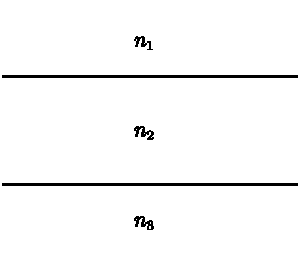
\includegraphics[scale=0.88]{等厚干涉示意.pdf}}
    \caption{等厚干涉示意图}\label{fig:等厚干涉示意}
\end{figure}


\begin{table}[H]
    \centering
    \caption{依据三种介质折射率判断在等厚干涉计算中是否需要附加光程差}
    \scalebox{0.90}{
      \begin{tabular}{ccc}
      \toprule
      {\sonti 类型} & $n_1>n_2>n_3${\sonti 或}$n_1<n_2<n_3$ & $n_1>n_2<n_3${\sonti 或}$n_1<n_2>n_3$ \\
      \midrule
      反射光干涉 & 无需附加$\frac{\lambda}{2}$ & 需附加$\frac{\lambda}{2}$ \\
      透射光干涉 & 需附加$\frac{\lambda}{2}$ & 无需附加$\frac{\lambda}{2}$ \\
      \bottomrule
      \end{tabular}}
    \label{tab:依据三种介质折射率判断在等厚干涉计算中是否需要附加光程差}
\end{table}

{\sonti 注意}:这里$\lambda$是指光在真空中的波长
\begin{itemize}
    \item {\sonti 杨氏双缝干涉}:杨氏双缝干涉实验是利用波阵面分割法来获得相干光的。用单色平行光照射一窄缝$S$,窄缝相当于一个线光源,$S$后放有与其平行且对称的两狭缝$S_1$与$S_2$,两缝之间距离$d$很小,两狭缝处在$S$发出光波的同一波阵面上,构成一对初相位相同的等强度的相干光源,在双缝的后面放置一个观察屏,可以在屏幕上观察到明暗相间的对称干涉条纹,这些条纹均与狭缝平行,条纹间距相等。设双缝之间的距离为$d$,双缝到屏的距离为$D$,如\textcolor{blue}{\cref{fig:杨氏双缝干涉}}所示。在屏上以屏中心为原点$O$,垂直于条纹方向建立$x$轴,用以表示干涉点的位置,设屏上坐标为$x$处的干涉点$P$到两缝的距离分别为$r_1$,$r_2$,且$D\gg x$,$D\gg d$
    \begin{figure}[H]
        \centerline{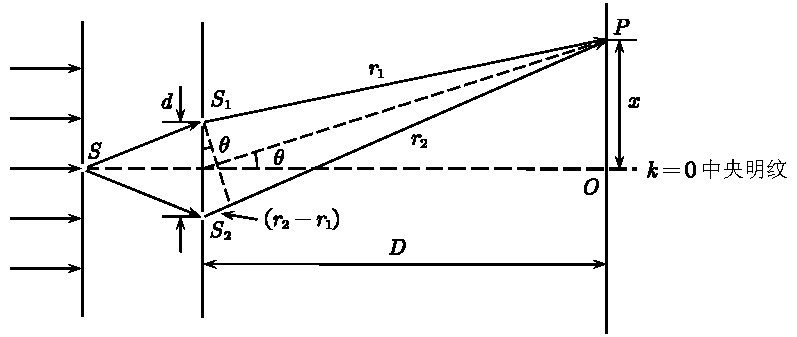
\includegraphics[scale=0.88]{杨氏双缝干涉.pdf}}
        \caption{杨氏双缝干涉实验示意图}\label{fig:杨氏双缝干涉}
    \end{figure}
    $$
    \Delta r=r_2-r_1=d\sin\theta=\left\{ \begin{array}{l}
        \pm 2k\cdot \frac{\lambda}{2},\text{明}\\
        \pm \left( 2k-1 \right) \cdot \frac{\lambda}{2},\text{暗}\\
    \end{array} \right. 
    $$
    $$
    \Delta r=d\sin\theta=d\tan\theta
    $$
    $$
    \left\{ \begin{array}{l}
        \sin \theta =\frac{\Delta r}{d}\\
        \tan \theta =\frac{x}{D}\\
    \end{array} \right. 
    $$
    $$
    x=D\tan\theta=D\sin\theta=\left\{ \begin{array}{l}
        \pm \frac{D}{d}\left[ 2k\cdot \frac{\lambda}{2} \right] ,\text{明}\\
        \pm \frac{D}{d}\left[ \left( 2k-1 \right) \cdot \frac{\lambda}{2} \right] ,\text{暗}\\
    \end{array} \right. 
    $$
    $k=0$对应于在点$O$处的零级明条纹,又称中央明纹。
    相邻明纹之间的距离,相邻暗纹之间的距离均为
    $$
    \Delta_\text{明}=\Delta_\text{暗}=\frac{D}{d}\lambda
    $$
    \item {\sonti 薄膜干涉}:薄膜干涉是利用振幅分割法来获得相干光的。薄膜干涉示意图如\textcolor{blue}{\cref{fig:薄膜干涉}}所示
    \begin{figure}[H]
        \centerline{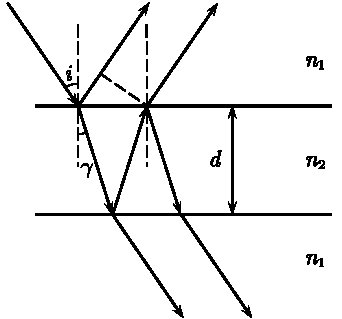
\includegraphics[scale=0.88]{薄膜干涉.pdf}}
        \caption{薄膜干涉示意图}\label{fig:薄膜干涉}
    \end{figure}
    对于反射光干涉情况,有
    $$
    \Delta=2d\sqrt{n_2^2-n_1^2\sin^2 i}+\frac{\lambda}{2}=\left\{ \begin{array}{l}
        k\lambda ,\text{加强}\\
        \left( 2k-1 \right) \cdot \frac{\lambda}{2},\text{减弱}\\
    \end{array} \right. 
    $$
    而对于折射光干涉情况,与上述恰好相反
    \begin{itemize}
        \item 增反膜:反射光增强
        \item 增透膜:透射光增强
    \end{itemize}
    \textbf{反射光与折射光互补},符合能量守恒
    \item {\sonti 劈尖(干涉)}:劈尖干涉示意图如\textcolor{blue}{\cref{fig:劈尖干涉}}所示。图中$\theta$很小,一般为$10^{-5}\sim 10^{-4}\,\mathrm{rad}$,因此在劈尖上表面处反射的光线和在劈尖下表面处反射的光线都可看作垂直于劈尖表面,由于劈尖层空气的折射率$n\left(n\thickapprox 1\right)$比玻璃的折射率$n_1$小,所以光在劈尖下表面反射时产生半波损失$\frac{\lambda}{2}$
    \begin{figure}[H]
        \centerline{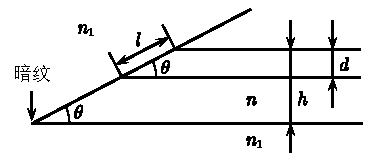
\includegraphics[scale=1.20]{劈尖干涉.pdf}}
        \caption{劈尖干涉示意图}\label{fig:劈尖干涉}
    \end{figure}
    上下表面反射的两相干光在劈尖厚度为$h$处的光程差为
    $$
    \Delta=2nh+\frac{\lambda}{2}\thickapprox 2h+\frac{\lambda}{2}=\left\{ \begin{array}{l}
        2k\cdot \frac{\lambda}{2},\text{明}\\
        \left( 2k-1 \right) \cdot \frac{\lambda}{2},\text{暗}\\
    \end{array} \right. 
    $$
    相邻明条纹之间的厚度差、相邻暗条纹之间的厚度差均为
    $$
    \Delta d=\frac{\lambda}{2n}\thickapprox \frac{\lambda}{2}
    $$
    相邻明条纹之间的距离、相邻暗条纹之间的距离均为
    $$
    \Delta l\thickapprox\frac{\Delta d}{\theta}=\frac{\lambda}{2n\theta}\thickapprox\frac{\lambda}{2\theta}
    $$
    $$
    \sin\theta=\frac{d}{l} \Rightarrow l=\frac{d}{\sin\theta}\thickapprox\frac{d}{\theta}
    $$
    在劈尖上方观察干涉图形是一些与棱边平行、均匀分布、明暗相间的直条纹。对于上述分析的劈尖,其棱边为暗纹;而对于别的劈尖,棱边明暗情况,涉及到半波损失的分析,与介质折射率排列的情况和观察方向有关,需要具体问题具体分析
    \begin{itemize}
        \item 当$\theta$减小时,条纹右移,条纹间距增大
        \item 当$\theta$增大时,条纹左移,条纹间距减小
    \end{itemize}
    \textbf{劈尖干涉可以用于判断工件表面的凹凸情况}:若劈尖开口朝右,从主视的俯视观察条纹,若条纹有一部分向左弯曲,则说明工件该处为凹槽;若条纹有一部分向右弯曲,则说明工件该处凸出

    若相邻明条纹之间的距离为$b$,对应空气膜厚度为差为$\frac{\lambda}{2}$,则间距为$a$对应的空气膜厚度差为$\frac{\lambda}{2}\cdot\frac{a}{b}=\frac{\lambda a}{2b}$
    \item {\sonti 牛顿环(干涉)}:一块曲率半径很大的平凸透镜与一平玻璃接触,构成一个上表面为球面,下表面为平面的空气劈尖,如\textcolor{blue}{\cref{fig:牛顿环}}所示
    \begin{figure}[H]
        \centerline{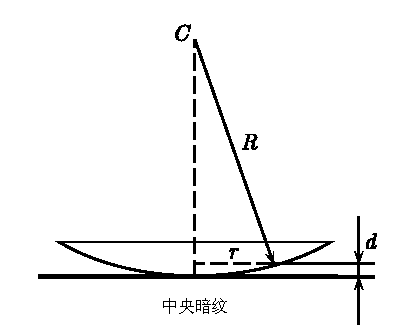
\includegraphics[scale=1.0]{牛顿环.pdf}}
        \caption{牛顿环示意图}\label{fig:牛顿环}
    \end{figure}
    可以观察到明暗相间的条纹,且中央为暗纹,条纹内圆疏,外圆密,条纹分布不均匀
    $$
    \Delta=2nd+\frac{\lambda}{2}\thickapprox 2d+\frac{\lambda}{2}=\left\{ \begin{array}{l}
        2k\cdot \frac{\lambda}{2},\text{明}\\
        \left( 2k-1 \right) \cdot \frac{\lambda}{2},\text{暗}\\
    \end{array} \right. 
    $$
    $$
    R^2=\left(R-d\right)^2+r^2,R\gg d \Rightarrow r=\sqrt{2dR}
    $$
    $$
    r=\left\{ \begin{array}{l}
        \sqrt{\frac{\left( k-\frac{1}{2} \right) R\lambda}{n}},\text{明}\\
        \sqrt{\frac{kR\lambda}{n}},\text{暗}\\
    \end{array} \right. 
    $$
    若将平凸透镜上移,则条纹中心收缩,条纹间距不变,环心呈明暗交替变化
    \item {\sonti 迈克尔孙干涉仪}:迈克尔孙干涉仪的主要优点在于它可以将两相干光束在空间完全分开(两光臂分布在互相垂直的方向上),便于在光路中安插待测样品或其他器件。光程差也可以通过移动反光镜$M_1$的方法来改变,$M_1$每移动$\frac{\lambda}{2}$的距离,光程差就改变一个波长,干涉场中就有一条明(或暗)条纹移过被认定为的参考点。条纹移动数目$N$与反光镜$M_1$移动的距离$\Delta d$之间的关系为
    $$
    \Delta d=N\cdot\frac{\lambda}{2}
    $$
    若$M_1$与$M_2$的距离为$d$增大,则干涉条纹从中心冒出并向外扩张,干涉条纹变密;若$d$减小,则干涉条纹向中心收缩,干涉条纹变稀
    
    若插入折射率为$n$的介质片,则有
    $$
    2nt-2t=N\lambda
    $$
    厚度为
    $$
    t=\frac{N\lambda}{2\left(n-1\right)}
    $$
\end{itemize}
\section{衍射}
\begin{itemize}
    \item {\sonti 夫琅禾费单缝衍射}:利用菲涅尔半波带法分析,如\textcolor{blue}{\cref{fig:夫琅禾费单缝衍射}}所示
    \begin{figure}[H]
        \centerline{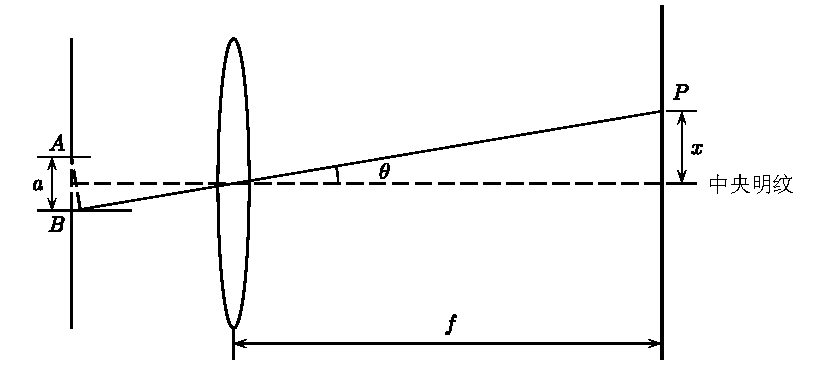
\includegraphics[scale=0.90]{夫琅禾费单缝衍射.pdf}}
        \caption{夫琅禾费单缝衍射示意图}\label{fig:夫琅禾费单缝衍射}
    \end{figure}
    单缝衍射的明纹(中心)、暗纹(中心)条件为
    $$
    a\sin\theta=\left\{ \begin{array}{l}
        0,\text{中央明纹}\\
        \pm 2k\cdot \frac{\lambda}{2},\text{暗}\\
        \pm \left( 2k-1 \right) \cdot \frac{\lambda}{2},\text{明}\\
    \end{array} \right. 
    $$
    $$
    x=f\tan\theta\thickapprox f\sin\theta
    $$
    $$
    x_\text{暗}=\frac{f}{a}\left[\pm 2k\cdot\frac{\lambda}{2}\right]
    $$
    $$
    x_\text{明}=\frac{f}{a}\left[\pm\left(2k-1\right)\cdot\frac{\lambda}{2}\right]
    $$
    定义相邻暗纹中心间的距离为条纹宽度,即
    $$
    \Delta x=\frac{f}{a}\cdot\lambda
    $$
    中央明纹宽度为
    $$
    x_0=2\cdot\frac{f}{a}\cdot\lambda=2\Delta x
    $$
    中央明纹最亮,各级明纹亮度随级数增大而减小
    
    当$\theta$增大时,$k$增大,半波带面积减小,所含子波数减少,子波振幅减小。$\theta$越大,分成的波带数也就越多
    \item {\sonti 圆孔衍射}:圆孔衍射图样是一系列明暗交替的同心圆环,中央是一个亮斑,称为艾里斑。若单色光博城为$\lambda$,圆孔直径为$D$,透镜的焦距为$f$,透镜光对焦平面上艾里斑的直径为$d$,所夹的平面角为$2\theta$,$\theta$为半角宽度,如\textcolor{blue}{\cref{fig:艾里斑}}所示。艾里斑的半角宽度满足下述关系:
    $$
    \theta=\frac{\frac{d}{2}}{f}=\frac{1.22\cdot\lambda}{D}
    $$
    \begin{figure}[H]
        \centerline{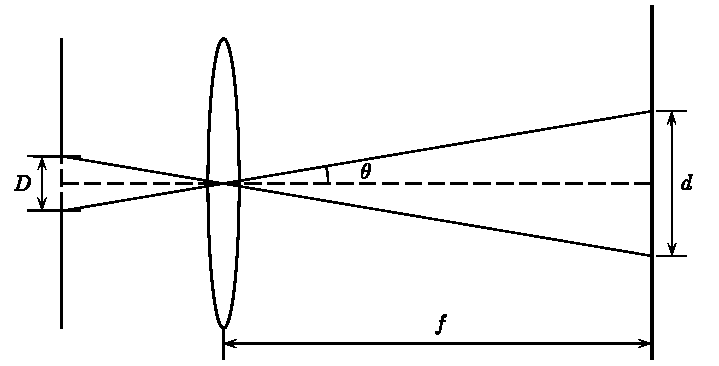
\includegraphics[scale=0.90]{艾里斑.pdf}}
        \caption{艾里斑}\label{fig:艾里斑}
    \end{figure}
    当两物点在透镜焦平面上形成的两个艾里斑中心的距离等于每一个艾里斑的半径时,认为两个物点刚好能被人眼或光学仪器所能分辨,这一条件称为\textbf{瑞利}{\sonti (Rayleigh)}\textbf{判据}。按瑞利判据可求出光学仪器能分辨的两物点的最小距离,恰能分辨时,两物点在透镜处所张的角称为\textbf{最小分辨角},用$\theta_0$表示,对应的正是艾里斑的半角宽度,如\textcolor{blue}{\cref{fig:瑞利判据}}所示
    \begin{figure}[H]
        \centerline{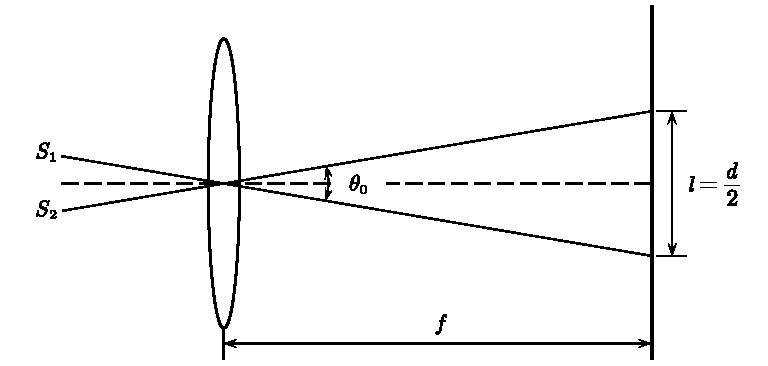
\includegraphics[scale=0.90]{瑞利判据.pdf}}
        \caption{瑞利判据}\label{fig:瑞利判据}
    \end{figure}
    因此有
    $$
    \theta_0=\frac{1.22\cdot\lambda}{D}
    $$
    将$\frac{1}{\theta_0}$定义为光学仪器的分辨本领,即
    $$
    \frac{1}{\theta_0}=\frac{D}{1.22\cdot\lambda}
    $$
    提高光学仪器的分辨本领可以加大物镜的通光孔径$D$,或者采用较短的工作波长$\lambda$
    \item {\sonti 光栅衍射}:不同狭缝光栅衍射结果不一样,随着狭缝的增多,明条纹亮度增大,明纹变细,相应的这些又细又亮的条纹之间的暗背景越来越暗。记$d=a+b$为光栅常量,$a$为透光的狭缝的宽度,$b$为刻痕宽度,此处因漫反射而不透光。光栅衍射明纹的形成示意图如\textcolor{blue}{\cref{fig:光栅衍射}}所示
    \begin{figure}[H]
        \centerline{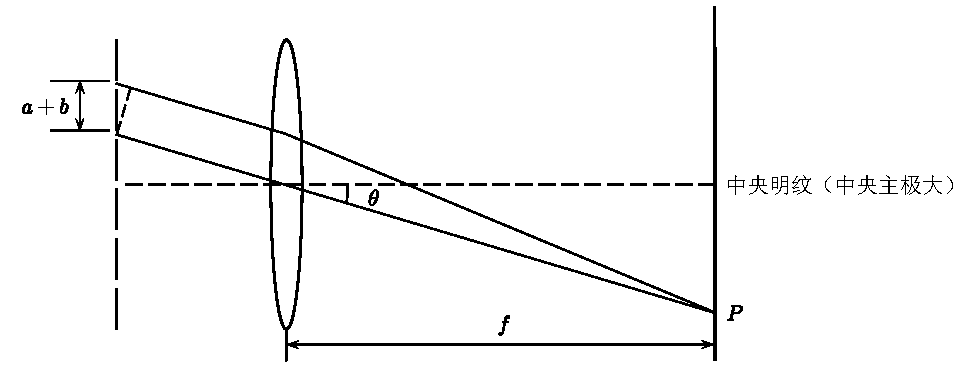
\includegraphics[scale=0.90]{光栅衍射.pdf}}
        \caption{光栅衍射明纹的形成示意图}\label{fig:光栅衍射}
    \end{figure}
    光栅方程:
    $$
    \left(a+b\right)\sin\theta=\pm k\lambda,k=0,1,2,\cdots
    $$
    若在某一衍射角为$\theta$的方向上,缝间子波干涉的光程差满足上式,则屏上出现明纹,称为光栅衍射主极大,式中$k$为主极大的级次,$k=0$对应于中央主极大
    \begin{itemize}
        \item 当$d$减小时,明纹间隔增大,条纹宽度减小:
        $$
        \sin\theta_1=\frac{\lambda}{d}
        $$
        $$
        \sin\theta_2=\frac{2\lambda}{d}
        $$
        因此,当$d$减小时,$\left(\theta_2-\theta_1\right)=\theta_1$增大,因此条纹间距增大
        \item 当$\lambda$增大时,明纹间隔增大
    \end{itemize}
    记狭缝数为$N$,则每两个主极大之间有$\left(N-1\right)$条暗纹,有$\left(N-2\right)$条次明纹;每两条暗纹之间有一条明纹,为次明纹
    
    \textbf{缺级现象}:考虑单缝衍射的效果,因此有
    $$
    \left\{ \begin{array}{l}
        \text{asin}\theta =\pm k'\lambda\\
        \left( a+b \right) \sin \theta =\pm k\lambda\\
    \end{array}\Rightarrow \frac{a}{a+b}=\frac{k}{k'} \right. 
    $$
    当多束干涉的主极大位置恰好为单缝衍射的暗纹中心时,这些主极大将在屏上消失,该现象称为缺级现象。由上式可以得出,当$\left(a+b\right)$与$a$的比为整数时,便有缺级现象
\end{itemize}
\section{光的偏振}
\textbf{只有横波才有偏振现象}

{\sonti 光振动的表示}:为简明地表示光的传播,常用于传播方向垂直的短线和点子分别表示在纸面内和垂直于纸面的光振动

{\sonti 自然光}:普通光源中各原子发光是独立的,每个波列的振幅、相位和振动方向都是随机的。光矢量具有均匀的轴对称分布,各方向光矢量振动的振幅相同。自然光并不能显示出偏振特性,这是由于光波的偏振性在每个方向都不占优势。其表示如\textcolor{blue}{\cref{fig:自然光}}所示
\begin{figure}[H]
    \centerline{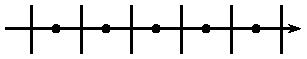
\includegraphics[scale=1.2]{自然光}}
    \caption{自然光的表示}
    \label{fig:自然光}
\end{figure}

{\sonti 完全偏振光}:光矢量只在一个固定平面内沿一个固定方向振动的光即为完全偏振光,也称\textbf{线偏振光},又称\textbf{平面偏振光}。其表示如\textcolor{blue}{\cref{fig:偏振光}}所示
\begin{figure}[H]
    \centerline{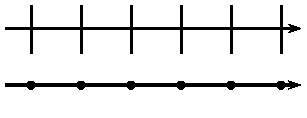
\includegraphics[scale=1.2]{偏振光}}
    \caption{偏振光的表示}
    \label{fig:偏振光}
\end{figure}

{\sonti 部分偏振光}:部分偏振光是介于线偏振光与自然光之间的一种光,例如将一束线偏振光与自然光混合,得到的光即为部分偏振光。其表示如\textcolor{blue}{\cref{fig:部分偏振光}}所示
\begin{figure}[H]
    \centerline{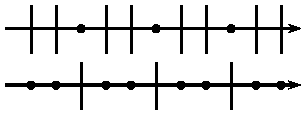
\includegraphics[scale=1.2]{部分偏振光}}
    \caption{部分偏振光的表示}
    \label{fig:部分偏振光}
\end{figure}
{\sonti 起偏与检偏}:
如\textcolor{blue}{\cref{fig:起偏与检偏}}所示,$P_1$与$P_2$为两个平行放置的偏振片,它们的偏振化方向分别用它们上面的虚平行线表示。当自然光垂直射于$P_1$时,透过的光将成为线偏振光,此时$P_1$用来产生偏振光,称之为起偏器。再使透过$P_1$形成的线偏振光入射于偏振片$P_2$,其可识别线偏振光的方向,因此$P_2$称为检偏器
\begin{figure}[H]
    \centerline{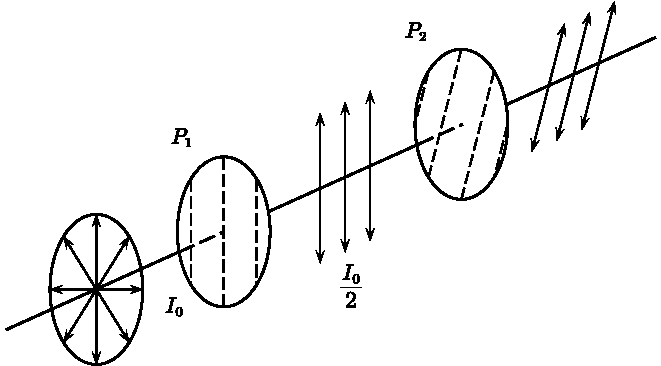
\includegraphics[scale=1.0]{起偏与检偏}}
    \caption{起偏与检偏}
    \label{fig:起偏与检偏}
\end{figure}

设自然光光矢量的光强为$I_0$,经过起偏器后,透过的光为线偏振光,其光强为$\frac{1}{2}I_0$

{\sonti 马吕斯定律}:设入射偏振光的光矢量为$A_1$,以$I_1$表示入射线偏振光的光强,振动方向与偏振片的偏振光方向成$\theta$角,透过检偏器后的光强为$I$,透过偏振片后光矢量振幅为$A$,则
$$
A=A_1\cos\theta
$$
又由于光强与振幅的平方成正比,则
$$
I=I_1\cos^2\theta
$$
\begin{example}
    自然光通过两个偏振化方向间成$\frac{\pi}{3}$角的偏振片,透射光强为$I$,现在这两块偏振片之间再插入另一偏振片,它的偏振化方向与上述两个偏振片均成$\frac{\pi}{3}$角,求透射光光强。

    \noindent\textbf{解}

    设入射光光强为$I_0$,则有
    $$
    I=\frac{1}{2}I_0\cos^2\frac{\pi}{3}
    $$

    因此入射光光强
    $$
    I_0=\left(\frac{1}{2}\right)^2\times2I=8I
    $$

    因此插入另一个偏振片后,投射光光强为
    $$
    I'=\frac{1}{2}I_0 \cos^2\frac{\pi}{6}\cdot\cos^2\frac{\pi}{6}=\frac{1}{2}\times8I\times\left(\frac{\sqrt{3}}{2}\right)^2\times\left(\frac{\sqrt{3}}{2}\right)^2=\frac{9}{4}I
    $$
\end{example}

{\sonti 反射和折射时光的偏振}

反射光、折射光一般不再为自然光,而是部分偏振光

反射光束中,垂直入射面的光矢量比平行入射面的要强,而折射光相反

一般情况下入射光、反射光、折射光如\textcolor{blue}{\cref{fig:一般反射折射}}所示
\begin{figure}[H]
    \centering
    \begin{minipage}{0.48\linewidth}
        \centering
        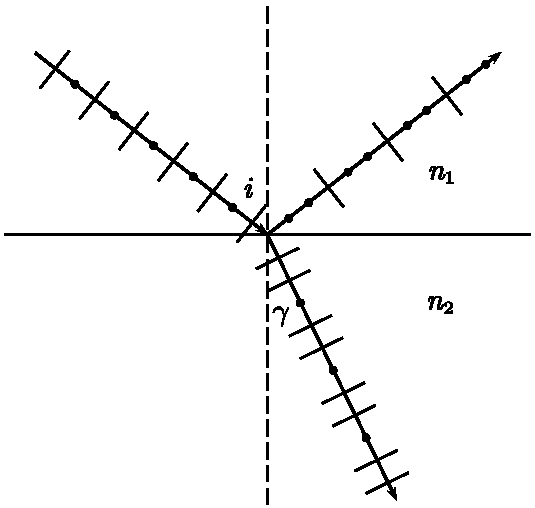
\includegraphics[scale=0.66]{一般反射折射.pdf}
        \caption{一般情况下光反射和折射时的偏振}
        \label{fig:一般反射折射}
    \end{minipage}
    %\qquad
    \begin{minipage}{0.48\linewidth}
        \centering
        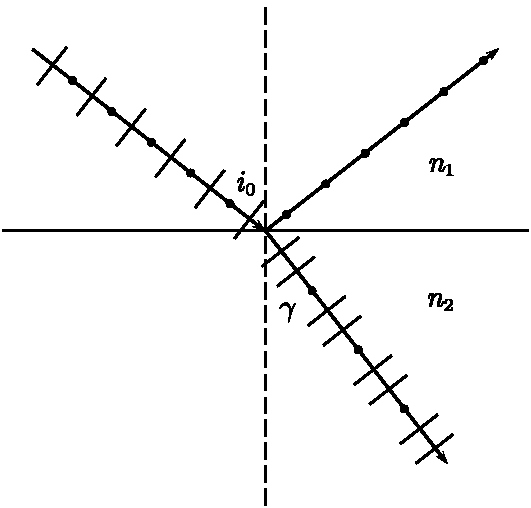
\includegraphics[scale=0.66]{布儒斯特角入射情况反射折射.pdf}
        \caption{布儒斯特角入射情况反射折射}
        \label{fig:布儒斯特角入射情况反射折射}
    \end{minipage}
\end{figure}

当入射角$i$与折射角$\gamma$之和为$\frac{\pi}{2}$,即反射光与折射光垂直时,反射光为光矢量垂直于入射面的线偏振光,如\textcolor{blue}{\cref{fig:布儒斯特角入射情况反射折射}}所示。这个特定的入射角称为起偏角,或称为\textbf{布儒斯特角}

若以$i_0$表示布儒斯特角,根据折射定律有
$$
n_1\sin i_0=n_2\sin\gamma
$$
式中$n_1$与$n_2$分别为介质$1$与介质$2$的折射率

此外有
$$
i_0+\gamma=\frac{\pi}{2} \Rightarrow \sin\gamma=\sin\left(\frac{\pi}{2}-i_0\right)=\cos i_0
$$

因此
$$
\tan i_0=\frac{n_2}{n_1}
$$
\chapter{气体动理论}
\newpage
\section{理想气体物态方程}
{\sonti 物态参量}:体积$V$,压强$p$,温度$T$
$$
1\,\mathrm{L}=1\,\mathrm{dm}^3=10^{-3}\,\mathrm{m}^3
$$
$$
1\,\mathrm{Pa}=1\,\mathrm{N}\cdot\mathrm{m}^{-2}
$$
$$
p=\frac{F}{S}
$$

通常,$45°$纬度海平面$0\,$\textcelsius 时大气压为$1\,\mathrm{atm}=1.013\times10^5\,\mathrm{Pa}$

{\sonti 水的三相点}(水、冰、水汽共存而达到平衡态)温度为$273.15\,\mathrm{K}$
$$
\frac{t}{\text{\textcelsius}}=\frac{T}{\mathrm{K}}-273.15
$$
$$
\frac{T}{\mathrm{K}}=\frac{t}{\text{\textcelsius}}+273.15
$$
$$
\frac{pV}{T}=\mathrm{C}
$$

{\sonti 理想气体}:压强不太大(与大气压相比),温度不太低(与室温相比)

{\sonti 标准状态}:$p_0=1.013\times 10^5\,\mathrm{Pa}$,$T_0=273.15\,\mathrm{K}$

在标准状态下,$1\mathrm{mol}$任何理想气体的体积均为$V_\mathrm{m}=22.4\,\mathrm{L}$

{\sonti 摩尔气体常量}:
$$
R=\frac{p_0V_0}{T_0}=8.31\,\mathrm{J}\cdot\mathrm{mol}^{-1}\cdot\mathrm{K}^{-1}
$$

对于物质的量为$\nu$,总质量为$m'$,摩尔质量为$M$的气体,理想气体物态方程为
$$
pV=\nu RT=\frac{m'}{M}RT
$$

记气体分子总数为$N$,阿伏伽德罗常数为$N_A=6.02\times10^{23}\,\mathrm{mol}^{-1}$,每一个分子的质量为$m$,则有
\begin{itemize}
    \item {\sonti 气体总质量}:$m'=Nm$
    \item {\sonti 摩尔质量}:$M=N_Am$
    \item {\sonti 物质的量}:$\nu=\frac{m'}{M}=\frac{mN}{mN_A}=\frac{N}{N_A}$
    \item {\sonti 分子数密度}:$n=\frac{N}{V}$
    \item {\sonti 气体密度}:$\rho=\frac{m'}{V}=\frac{mN}{\frac{N}{n}}=mn$
\end{itemize}
\begin{eqnarray}
    pV&=&\nu RT \nonumber      \\
    ~&=&\frac{m'}{M}RT \nonumber    \\
    ~&=&\frac{m'}{mN_A}RT \nonumber		\\
    ~&=&N\frac{R}{N_A}T \nonumber
\end{eqnarray}

{\sonti 玻尔兹曼常量}:
$$
k=\frac{R}{N_A}=1.38\times10^{-23}\,\mathrm{J}\cdot\mathrm{K}^{-1}
$$

理想气体物态方程还可写为
$$
pV=NkT
$$
$$
p=\frac{N}{V}kT=nkT
$$
\section{物质的微观模型、统计规律}
物质结构的分子、原子学说:
\begin{itemize}
    \item 一切宏观物体都是由大量分子或原子组成
    \item 分子间有力的相互作用
    \item 分子永不停息地作无规则的热运动
\end{itemize}
$$
1\,\mathring{\mathrm{A}}=0.1\,\mathrm{nm}
$$

当系统在无外界作用时,处于平衡态下的气体密度是均匀的。大量分子沿空间各方向运动的机会相等,沿各方向运动的分子数相等,分子速度在各方向上分量的各种平均值也相等
\section{理想气体的压强公式}
对于气体分子的速度,有以下关系:
$$
\overline{v^2}\ne \left(\overline{v}\right)^2
$$
$$
\overline{v^2}=\overline{v_x^2}+\overline{v_y^2}+\overline{v_z^2}
$$
$$
\overline{v_x^2}=\overline{v_y^2}=\overline{v_z^2}=\frac{1}{3}\overline{v^2}
$$

{\sonti 理想气体压强公式}:
$$
p=\frac{1}{3}nm\overline{v^2}=\frac{2}{3}n\left(\frac{1}{2}m\overline{v^2}\right)
$$

{\sonti 分子平均平动能}:
$$
\overline{\varepsilon_\mathrm{kt}}=\frac{1}{2}m\overline{v^2}
$$
因此,理想气体压强还可写为
$$
p=\frac{2}{3}n\overline{\varepsilon_\mathrm{kt}}
$$

对于理想气体,有$\overline{\boldsymbol{v}}=0$

分子数密度越大,分子的平均平动能就越大,压强也就越大
\section{理想气体的温度公式}
由理想气体的物态方程和压强公式
$$
\left\{ \begin{array}{l}
	p=nkT\\
	p=\frac{2}{3}n\overline{\varepsilon _\mathrm{kt}}\\
\end{array} \right. 
$$
可以得到
$$
\overline{\varepsilon _\mathrm{kt}}=\frac{1}{2}m\overline{v^2}=\frac{3}{2}kT
$$

{\sonti 气体的方均根速率}:
$$
v_\mathrm{r}=\sqrt{\overline{v^2}}=\sqrt{3}\sqrt{\frac{kT}{m}}=\sqrt{3}\sqrt{\frac{RT}{M}}
$$
\section{能量均分定理}
单原子、刚性双原子、刚性多原子分子自由度,见\textcolor{blue}{\cref{tab:FreeDegree}}
\begin{table}[H]
    \centering
    \caption{单原子、刚性双原子、刚性多原子分子自由度}
    \scalebox{0.90}{
      \begin{tabular}{cccc}
      \toprule
      {\sonti 分子类型} & {\sonti $t$(平动自由度)} & {\sonti $r$(转动自由度)} & {\sonti $i$(总自由度)} \\
      \midrule
      单原子   & 3     & 0     & 3 \\
      刚性双原子 & 3     & 2     & 5 \\
      刚性多原子 & 3     & 3     & 6 \\
      \bottomrule
      \end{tabular}}
    \label{tab:FreeDegree}
\end{table}

{\sonti 能量均分定理}:在温度为$T$的平衡态下,气体分子任何一个自由度的平均动能都相等,均为$\frac{1}{2}kT$

气体分子的平均动能与平均平动动能、平均转动动能的关系为
$$
\overline{\varepsilon_\mathrm{k}}=\overline{\varepsilon_\mathrm{kt}}+\overline{\varepsilon_\mathrm{kr}}
$$

{\sonti 理想气体的平均能量}:$\overline{\varepsilon}=\frac{i}{2}kT$
\section{理想气体的内能}
{\sonti 气体内能}=所有分子热运动的{\sonti 动能}+分子间相互作用的{\sonti 势能}

{\sonti 理想气体的内能}=分子热运动的{\sonti 动能}

这是由于理想气体分子间无相互作用力,即分子间无势能

{\sonti 理想气体的内能}:
$$
E=\frac{i}{2}\nu RT=\frac{i}{2}pV
$$

理想气体的内能完全取决于气体的温度$T$和气体分子的自由度$i$。对于给定的理想气体,其内能为温度$T$的单值函数,即$E=E\left(T\right)$,因此有
$$
\mathrm{d}E=\frac{i}{2}\nu R\mathrm{d}T
$$
\section{麦克斯韦气体分子速率分布律}
{\sonti 气体分子的速率分布函数}:
$$
f\left(v\right)=\frac{1}{N}\frac{\mathrm{d}N}{\mathrm{d}v}
$$
表示在速率$v$附近单位速率区间内的分子数占总分子数的百分比;也可表述为任一单个分子在速率$v$附近单位速率区间内出现的概率,因此$f\left(v\right)$又称概率密度

速率分布曲线下微元面积为
$$
f\left(v\right)\mathrm{d}v=\frac{\mathrm{d}N}{N}
$$
其表示速率$v$附近$\mathrm{d}v$区间内的分子数占总分子数的百分比。而介于$v_1$与$v_2$之间的分子数$\Delta N$占总分子数$N$的百分比,即速率分布曲线下$v_1$与$v_2$之间的面积为
$$
\frac{\Delta N}{N}=\int_{v_1}^{v_2}f\left(v\right)\mathrm{d}v
$$

速率分布曲线下面积为分布在$v=0$到$v=\infty$整个速率区间内的分子数全部百分比之和,显然该值为$1$,即
$$
\int_{0}^{\infty}f\left(v\right)\mathrm{d}v=1
$$

{\sonti 气体分子的速率分布函数的应用}:在$v_1$到$v_2$之间
\begin{itemize}
    \item 分子数:$\int_{v_1}^{v_2}Nf\left(v\right)\mathrm{d}v=N\int_{v_1}^{v_2}f\left(v\right)\mathrm{d}v$
    \item 速率之和:$\int_{v_1}^{v_2}vNf\left(v\right)\mathrm{d}v=N\int_{v_1}^{v_2}vf\left(v\right)\mathrm{d}v$
    \item 动能之和:$\int_{v_1}^{v_2}\frac{1}{2}mv^2Nf\left(v\right)\mathrm{d}v=N\int_{v_1}^{v_2}\frac{1}{2}mv^2f\left(v\right)\mathrm{d}v$
\end{itemize}

{\sonti 麦克斯韦速率分布律}:
$$
\frac{\mathrm{d}N}{N}=f\left(v\right)\mathrm{d}v=4\pi\left(\frac{m}{2\pi kT}\right)^{\frac{3}{2}}v^2\mathrm{e}^{-\frac{mv^2}{2\pi kT}}\mathrm{d}v
$$

{\sonti 分子热运动的三种统计速率}:
\begin{itemize}
    \item {\sonti 方均根速率}:$v_\mathrm{r}=\sqrt{\overline{v^2}}$
    $$
    v_\mathrm{r}=\sqrt{3}\sqrt{\frac{kT}{m}}=\sqrt{3}\sqrt{\frac{RT}{M}}
    $$
    \item {\sonti (算数)平均速率}:$v_\mathrm{a}=\overline{v}$
    $$
    v_\mathrm{a}=\sqrt{\frac{8}{\pi}}\sqrt{\frac{kT}{m}}=\sqrt{\frac{8}{\pi}}\sqrt{\frac{RT}{M}}
    $$
    \item {\sonti 最概然速率}:$v_\mathrm{p}$,为$f\left(v\right)$的极大值
    $$
    v_\mathrm{p}=\sqrt{2}\sqrt{\frac{kT}{m}}=\sqrt{2}\sqrt{\frac{RT}{M}}
    $$
\end{itemize}
因此,三者的大小关系为$v_\mathrm{r}>v_\mathrm{a}>v_\mathrm{p}$
\section{分子平均碰撞频率、平均自由程}
{\sonti 分子平均碰撞频率}:$\overline{Z}$,表示一个分子每秒内与其他分子平均碰撞的次数

{\sonti 平均自由程}:$\overline{\lambda}$,表示每两次碰撞之间一个分子自由运动的平均路程

两者有如下关系:
$$
\overline{\lambda}=\frac{\overline{v}}{\overline{Z}}=\frac{v_\mathrm{a}}{\overline{Z}}
$$
其中$\overline{v}=v_\mathrm{a}$为平均速率

由上式,可得到如下结论:$\overline{Z}$越大,分子碰撞越频繁,$\overline{\lambda}$越小

{\sonti 分子的平均碰撞频率}:
$$
\overline{Z}=\sqrt{2}\pi d^2 v_\mathrm{a} n
$$

{\sonti 分子的平均自由程}:
$$
\overline{\lambda}=\frac{v_\mathrm{a}}{\overline{Z}}=\frac{1}{\sqrt{2}\pi d^2 n}
$$
其中,$d$为分子直径,$n$为分子数密度

由上式,可得到如下结论:分子直径越大,分子运动时越容易与其他分子发生碰撞,两次碰撞间分子运动的自由距离越短,即分子平均自由程越小

由$p=nkT$,即$n=\frac{p}{kT}$,可得到
$$
\overline{\lambda}=\frac{kT}{\sqrt{2}\pi d^2 p}
$$
\chapter{热力学基础}
\newpage
\section{名词解释}
{\sonti 非平衡过程(非静态过程)}:系统在整个过程中将经历一系列的非平衡态,这样的过程称为\textbf{非平衡过程}{\sonti (}\textbf{非静态过程}{\sonti )}

{\sonti 准静态过程}:如果系统在过程进行中,每一个中间状态的变化进行得无限缓慢,使得任意时刻所经历的中间状态都无限地接近平衡态,则这样的过程称为\textbf{准静态过程}。准静态过程是理想化、抽象化的

{\sonti 功}:功是过程量,用$W$表示
$$
\mathrm{d}W=p\mathrm{d}V
$$

当$\mathrm{d}W>0$时,气体膨胀,系统对外做正功

当$\mathrm{d}W<0$时,气体收缩,系统对外做负功(外界对气体做正功)
$$
W=\int_V p\mathrm{d}V=\int_{V_1}^{V_2} p\mathrm{d}V
$$

{\sonti 内能}:内能是状态量,用$E$表示

理想气体的内能仅是\textbf{温度}的函数,由于$E=\frac{i}{2}\nu RT$

内能=动能+势能

系统内能的改变完全取决于系统的始末状态,与过程无关,$\Delta E=E_2-E_1$

对于理想气体(压强不太大,温度不太低)而言,其内能仅有分子动能决定,由于理想气体分子间无相互作用力,$E=\frac{i}{2}\nu RT$

{\sonti 热量}:热量是过程量,用$Q$表示,传热过程中传递的能量称为热量

若需要改变系统的状态或者内能,需要\textbf{对系统做功}或者\textbf{向气体传递热量}
\section{热力学第一定律}
\textbf{第一类永动机是不可能实现的}

{\sonti 热力学第一定律}:系统从外界吸收的热量,一部分使系统的内能增加,另一部分使系统对外界做功,即
$$
Q=\Delta E+W
$$

系统从外界吸收热量,$Q>0$

系统向外界释放热量,$Q<0$

系统对外界做功,$W>0$

外界对系统做功,$W<0$

热力学第一定律还可写为
$$
\mathrm{d}Q=\mathrm{d}E+\mathrm{d}W=\mathrm{d}E+p\mathrm{d}V
$$

\section{理想气体的等值过程}
{\sonti 等容过程}:$\mathrm{d}V=0$
$$
\mathrm{d}V=0 \Rightarrow \mathrm{d}W=p\mathrm{d}V=0
$$
$$
\mathrm{d}Q_V=\mathrm{d}E+\mathrm{d}W=\mathrm{d}E=\frac{i}{2}\nu R\mathrm{d}T
$$
$$
Q_V=E_2-E_1=\frac{i}{2}\nu R(T_2-T_1)
$$

{\sonti 等压过程}:$\mathrm{d}p=0$
$$
\left. \begin{array}{r}
	pV=\nu RT\\
	\mathrm{d}\left( pV \right) =p\mathrm{d}V+V\mathrm{d}p\\
	\mathrm{d}\left( \nu RT \right) =\nu R\mathrm{d}T\\
\end{array} \right\} \Rightarrow p\mathrm{d}V+V\mathrm{d}p=\nu R\mathrm{d}T
$$
$$
\left. \begin{array}{r}
	p\mathrm{d}V+V\mathrm{d}p=\nu R\mathrm{d}T\\
	\mathrm{d}p=0\\
\end{array} \right\} \Rightarrow p\mathrm{d}V=\nu R\mathrm{d}T
$$
$$
\mathrm{d}Q_p=\mathrm{d}E+\mathrm{d}W=\mathrm{d}E+p\mathrm{d}V=\frac{i}{2}\nu R\mathrm{d}T + \nu R\mathrm{d}T
$$
$$
Q_p=\frac{i}{2}\nu R(T_2-T_1)+\nu R(T_2-T_1)
$$

{\sonti 等温过程}:$\mathrm{d}T=0 \Rightarrow \mathrm{d}E=0$
$$
\mathrm{d}Q_T=\mathrm{d}E+\mathrm{d}W=\mathrm{d}W=p\mathrm{d}V
$$
$$
pV=\nu RT \Rightarrow p=\nu RT\cdot \frac{1}{V}
$$
$$
\mathrm{d}W=p\mathrm{d}V=\nu RT\cdot \frac{1}{V}\mathrm{d}V
$$
$$
Q_T=W=\int_{V_1}^{V_2} \nu RT\cdot \frac{1}{V}\mathrm{d}V =\nu RT\ln \frac{V_2}{V_1}
$$
$$
\frac{p_1V_1}{T}=\frac{p_2V_2}{T} \Rightarrow Q_T=\nu RT\ln \frac{p_1}{p_2}
$$
\section{气体的摩尔热容}
{\sonti 热容}:$C=\frac{\mathrm{d}Q}{\mathrm{d}T}$,$\mathrm{J}\cdot\mathrm{K}^{-1}$

{\sonti 摩尔热容}:$C_\mathrm{m}=\frac{\mathrm{d}Q}{\nu \mathrm{d}T}$,$\mathrm{J}\cdot\mathrm{mol}^{-1}\cdot\mathrm{K}^{-1}$

{\sonti 比热容}:$c=\frac{\mathrm{d}Q}{m'\mathrm{d}T}=\frac{C}{m'}$,$\mathrm{J}\cdot\mathrm{kg}^{-1}\cdot\mathrm{K}^{-1}$

$$
C_\mathrm{m}=\frac{\mathrm{d}Q}{\nu \mathrm{d}T}=\frac{\mathrm{d}E+p\mathrm{d}V}{\nu\mathrm{d}T}
$$

{\sonti 理想气体的摩尔定容热容}:

$$
\mathrm{d}V=0 \Rightarrow \mathrm{d}W=p\mathrm{d}V=0
$$
$$
C_{V,\mathrm{m}}=\frac{\mathrm{d}Q_V}{\nu \mathrm{d}T}=\frac{\mathrm{d}E}{\nu\mathrm{d}T}=\frac{\frac{i}{2}\nu R\mathrm{d}T}{\nu\mathrm{d}T}=\frac{i}{2}R
$$
由此,可得到:
$$
\mathrm{d}E=\nu\cdot C_{V,\mathrm{m}}\cdot \mathrm{d}T
$$
$$
\int_{E_1}^{E_2}\mathrm{d}E=\int_{T_1}^{T_2}\nu\cdot C_{V,\mathrm{m}}\cdot \mathrm{d}T \Rightarrow \Delta E=E_2-E_1=\nu\cdot C_{V,\mathrm{m}}\cdot\left(T_2-T_1\right)
$$

{\sonti 理想气体的摩尔定压热容}:
$$
\mathrm{d}p=0 \Rightarrow V\mathrm{d}p=0 \Rightarrow p\mathrm{d}V=\nu R\mathrm{d}T
$$
$$
C_{p,\mathrm{m}}=\frac{\mathrm{Q}_p}{\nu \mathrm{d}T}=\frac{\mathrm{d}E+p\mathrm{d}V}{\nu \mathrm{d}T}=\frac{\frac{i}{2} \nu R\mathrm{d}T+\nu R\mathrm{d}T}{\nu \mathrm{d}T}
$$
$$
C_{p,\mathrm{m}}=\frac{i}{2}R+R=C_{V,\mathrm{m}}+R
$$
$$
C_{p,\mathrm{m}}-C_{V,\mathrm{m}}=R
$$
$$
C_{p,\mathrm{m}}>C_{V,\mathrm{m}}
$$
$$
\mathrm{d}Q_p=\nu\cdot C_{p,\mathrm{m}} \cdot \mathrm{d}T \Rightarrow Q_p=\nu\cdot C_{p,\mathrm{m}}\cdot\left(T_2-T_1\right)
$$

{\sonti 比热容比}:$\gamma =\frac{C_{p,\mathrm{m}}}{C_{V,\mathrm{m}}}=\frac{\frac{i}{2}R+R}{\frac{i}{2}R}=\frac{i+2}{i}>1$
\begin{itemize}
    \item {\sonti 单原子分子气体}:$\gamma = \frac{5}{3}$
    \item {\sonti 刚性双原子分子气体}:$\gamma = \frac{7}{5}$
    \item {\sonti 刚性多原子分子气体}:$\gamma = \frac{8}{6}=\frac{4}{3}$
\end{itemize}
\section{理想气体的绝热过程}
在理想气体的绝热过程中,有$\mathrm{d}Q=0$,因此$\mathrm{d}E+p\mathrm{d}V=0$

{\sonti 理想气体的绝热过程方程}:
$$
pV^\gamma=\mathrm{const}
$$
$$
V^{\gamma-1}T=\mathrm{const}
$$
$$
p^{\gamma-1}T^{-\gamma}=\mathrm{const}
$$
$$
V^{\gamma-1}E=\mathrm{const}
$$

绝热线与等温线的比较见\textcolor{blue}{\cref{fig:绝热线与等温线的比较}},可以发现\textbf{绝热线比等温线更陡}
\begin{figure}[H]
    \centerline{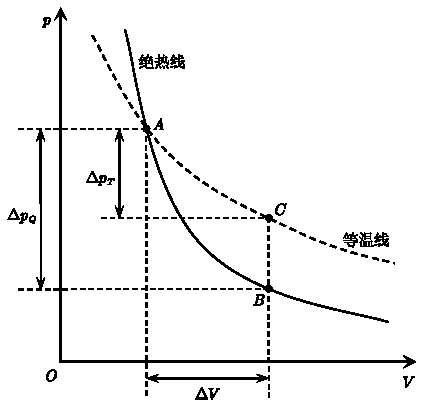
\includegraphics[scale=1.2]{绝热线与等温线的比较.pdf}}
    \caption{绝热线与等温线的比较}\label{fig:绝热线与等温线的比较}
\end{figure}
\section{循环过程}
系统经历一个循环之后,其内能并没有改变,即$\Delta E=0$

在$p-V$图中,顺时针方向进行的为正循环,即热机;逆时针方向进行的为逆循环,即制冷机

{\sonti 正循环}:
\begin{figure}[H]
    \centerline{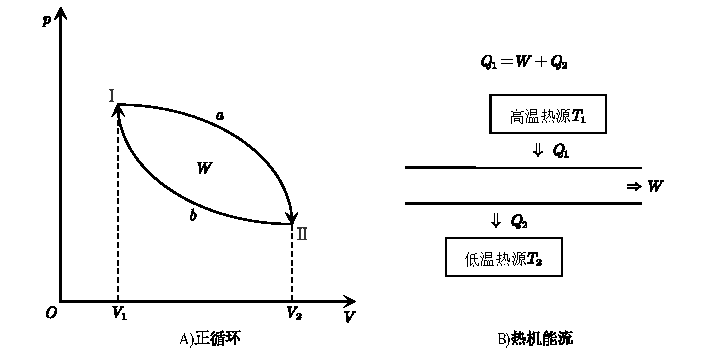
\includegraphics[scale=1.2]{正循环与热机能流图.pdf}}
    \caption{正循环与热机能流图}\label{fig:正循环与热机能流图}
\end{figure}
\hspace*{2em}{\sonti 热机效率}:$\eta=\frac{W}{Q_1}=\frac{Q_1-Q_2}{Q_1}=1-\frac{Q_2}{Q_1}$

{\sonti 逆循环}:
\begin{figure}[H]
    \centerline{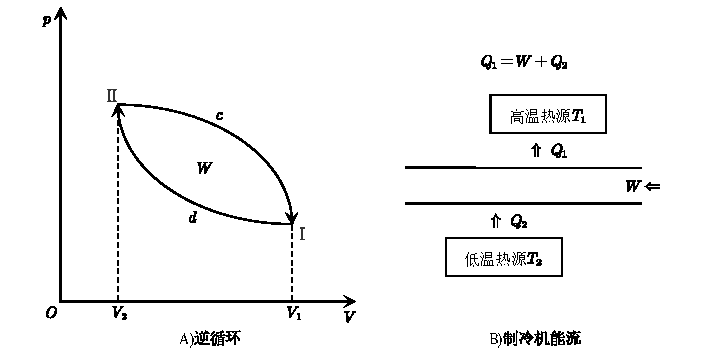
\includegraphics[scale=1.2]{逆循环与制冷机能流图.pdf}}
    \caption{逆循环与制冷机能流图}\label{fig:逆循环与制冷机能流图}
\end{figure}
\hspace*{2em}{\sonti 制冷系数}:$e=\frac{Q_2}{W}=\frac{Q_2}{Q_1-Q_2}$

{\sonti 卡诺循环}:

卡诺循环是由两个等温过程以及两个绝热过程组合而成,其工作过程如\textcolor{blue}{\cref{fig:卡诺循环}}所示。其中$1\to2$为等温过程;$2\to3$为绝热过程;$3\to4$为等温过程;$4\to1$为绝热过程
\begin{figure}[H]
    \centerline{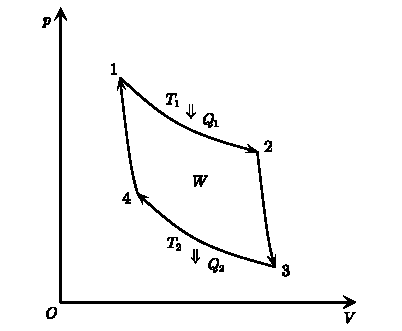
\includegraphics[scale=1.2]{卡诺循环.pdf}}
    \caption{卡诺循环}\label{fig:卡诺循环}
\end{figure}
对于上图,有如下结论:
$$
\frac{Q_2}{Q_1}=\frac{T_2}{T_1}
$$
$$
\frac{V_2}{V_1}=\frac{V_3}{V_4}
$$
$$
\eta=1-\frac{Q_2}{Q_1}=1-\frac{T_2}{T_1}=\frac{T_1-T_2}{T_1}
$$

{\sonti 卡诺逆循环}:
$$
e=\frac{Q_2}{W}=\frac{Q_2}{Q_1-Q_2}=\frac{T_2}{T_1-T_2}
$$

\textbf{若两个热源的$\Delta T$越大,卡诺循环的效率就越高}

{\sonti 卡诺定理}:
\begin{itemize}
    \item 在相同的高温热源与低温热源之间工作的任意工质的可逆机,它们的效率均相等,即$\eta=1-\frac{T_2}{T_1}$
    \item 工作在相同的高温热源与低温热源之间的一切不可逆机的效率都不可能大于在同样两热源之间的可逆机的效率,即$\eta'\leqslant 1-\frac{T_2}{T_1}$
\end{itemize}
\section{热力学第二定律}
\textbf{第二类永动机是不可能实现的}

{\sonti 热力学第二定律的两种表述}:
\begin{itemize}
    \item {\sonti 开尔文表述}:不可能制造出这样一种循环工作的热机,它只从单一热源吸收热量来做功而不放出热量给其他物体,或者说不使外界发生任何变化
    \item {\sonti 克劳修斯表述}:不可能把热量从低温物体自动向高温物体传递而不引起外界的变化
\end{itemize}

{\sonti 热力学第二定律的统计意义}:在一个不受外界影响的孤立系统中发生的一切实际过程,都是从概率小(微观态数少)的宏观态向概率大(微观态数多)的宏观态进行。与之相反的过程,并非绝对不可能发生,只是由于概率极小,实际上是观察不到的。此外,其还表明了它的适用范围只能是由大量微观粒子组成的宏观系统,对于粒子数很少的系统则是没有意义的
\section{熵}
热力学第二定律还可表述为在孤立系统中所进行的自然过程总是沿着熵增大的方向进行,它是不可逆的。平衡态对应的是熵最大的状态。这种表述称为\textbf{熵增加原理},其表达式为
$$
\Delta S>0
$$

若孤立系统经历的是可逆过程,则意味着过程中任意两个状态的热力学概率都相等,因而熵保持不变,有$\Delta S=0$,结合上述,有$\Delta S \geqslant 0$,它表明:\textbf{孤立系统内无论进行什么过程,系统的熵永不减少}
\chapter{静电场}
\newpage
\section{电荷}
原子是由\textbf{一个带正电的原子核}和\textbf{若干个绕核运动的带负电的电子}组成;原子核由\textbf{带正电的质子}和\textbf{不带电的中子}组成。整个原子呈电中性,物体表现为不带电

用丝绢摩擦玻璃棒之后,失去电子的玻璃棒带正电,获得电子的丝绢带负电

{\sonti 电荷的量子化}

电子的比荷(核质比)为$\frac{e}{m}$

带电体的电荷量是电子电荷的整数倍,以$e$为电子的电荷绝对值,则带电体的电荷量为$q=\pm ne$,$n$为整数

{\sonti 电荷守恒定律}:在一个孤立带电系统中,即没有静电荷通过系统界面,无论发生怎样的物理过程与化学过程,系统所具有的正负电荷的代数和总是保持不变
\section{库仑定律}
{\sonti 点电荷}:带电体的线度与其他有关长度相比可忽略不计,即带电体可以看作只有电荷的几何点。点电荷为物理模型,实际上不存在

{\sonti 库仑定律}:同号电荷相斥,异号电荷相吸。静止电荷之间的作用力称作库仑力
$$
\boldsymbol{F}=\frac{1}{4\pi \varepsilon _0}\frac{q_1q_2}{r^2}\boldsymbol{e}_r
$$
其中,$\boldsymbol{e}_r$为方向矢量,沿径向;$\varepsilon _0$为真空电容率,其值为
$$
\varepsilon _0=8.85\times 10^{-12}\,\mathrm{C}^2\cdot\mathrm{N}^{-1}\cdot\mathrm{m}^{-2}
$$
此外,有
$$
\frac{1}{4\pi \varepsilon _0}=9.0\times10^{9}\,\mathrm{C}^{-2}\cdot\mathrm{N}\cdot\mathrm{m}^{2}
$$

对于两个以上的点电荷相互作用时利用静电力的叠加原理,矢量计算,满足平行四边形定则
\section{电场强度}
由静止电荷所激发的电场称为静电场,该电荷称为场源电荷。静电场是电磁场的一种特殊形态,电磁场与实物物质一样具有能量、质量、动量等

{\sonti 试验电荷}:需要满足两个条件,电荷量足够小;几何线度足够小

{\sonti 电场强度}:$\boldsymbol{E}=\frac{\boldsymbol{F}}{q_0}$,$\mathrm{N}\cdot\mathrm{C}^{-1}$或$\mathrm{V}\cdot\mathrm{m}^{-1}$

只要有电荷存在,就有电场存在,电场是客观存在的。电场强度是空间位置的函数

对于\textbf{点电荷的电场强度}的计算,利用矢量求和,即
$$
\boldsymbol{E}=\sum_{i=1}^{n}\boldsymbol{E}_i
$$
设真空中有一点电荷$Q$,在离该电荷$r$处的$P$点的场强为$\boldsymbol{E}=\frac{Q}{4\pi\varepsilon_0r^2}\boldsymbol{e}_r$

对于\textbf{连续带电体的电场强度}的计算,利用积分求和。针对不同题型,利用下述三式中的某一个,即
$$
\mathrm{d}q=\lambda \mathrm{d}l
$$
$$
\mathrm{d}q=\sigma \mathrm{d}S
$$
$$
\mathrm{d}q=\rho \mathrm{d}V
$$

\begin{example}
    一均匀带电的细棒,长度为$L$,电荷线密度为$\lambda$,求在细棒中垂线上与细棒距离为$a$的场点处的电场强度。{\sonti (仅需记住结论即可)}
    \begin{figure}[H]
        \centerline{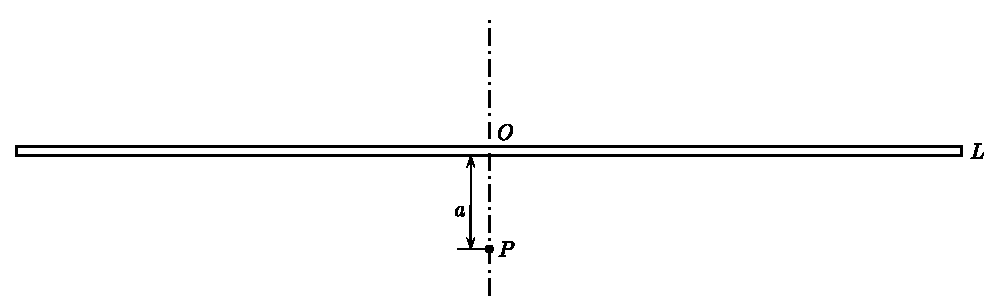
\includegraphics[scale=0.8]{CH09EX01.pdf}}
    \end{figure}
    \noindent\textbf{解}

    场强的大小为
    $$
    E_P=\frac{1}{4\pi\varepsilon_0}\frac{\lambda L}{a\sqrt{\frac{L^2}{4}+a^2}}
    $$
    
    场强的方向垂直于带电细棒
    
    当电荷为正时,由细棒指向外;当电荷为负时,由细棒指向内
    
    {\sonti 讨论两种特殊情况}:
    \begin{itemize}
        \item $a\gg L$,$E_P=\frac{1}{4\pi\varepsilon_0}\frac{\lambda L}{a^2}$
        \item $a\ll L$,$E_P=\frac{1}{2\pi\varepsilon_0}\frac{\lambda}{a}$
    \end{itemize}
\end{example}
\newpage
\begin{example}
    设电荷$q$均匀分布在半径为$R$的圆环上,计算在环的轴线上与环心相距为$x$的$P$点的场强。

    \noindent\textbf{解}
    \begin{figure}[H]
        \centerline{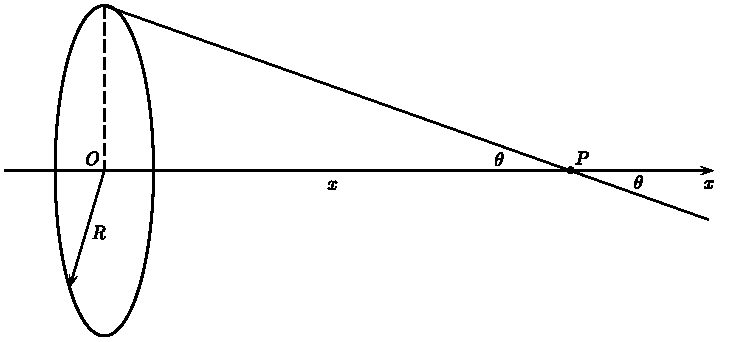
\includegraphics[scale=1.0]{CH09EX02.pdf}}
    \end{figure}
    $$
    \mathrm{d}E=\frac{1}{4\pi\varepsilon_0}\frac{\lambda \mathrm{d}l}{r^2}=\frac{\lambda \mathrm{d}l}{4\pi\varepsilon_0\left(x^2+R^2\right)}
    $$
    $$
    \cos\theta=\frac{x}{\sqrt{x^2+R^2}}
    $$
    $$
    \lambda=\frac{q}{2\pi R}
    $$
    
    由于$E_\bot$相互抵消,则$E=E_\parallel$
    $$
    \mathrm{d}E_\parallel=\mathrm{d}E\cdot\cos\theta=\frac{x\lambda\mathrm{d}l}{4\pi\varepsilon_0\left(x^2+R^2\right)^{\frac{3}{2}}}
    $$
    
    因此
    \begin{eqnarray}
        E=\int\mathrm{d}E_\parallel &=&\int_{0}^{2\pi R}\frac{x\lambda}{4\pi\varepsilon_0\left(x^2+R^2\right)^{\frac{3}{2}}}\mathrm{d}l \nonumber \\
        ~&=&\frac{x\lambda\cdot 2\pi R}{4\pi\varepsilon_0\left(x^2+R^2\right)^{\frac{3}{2}}} \nonumber \\
        ~&=&\frac{\frac{q}{2\pi R}\cdot 2\pi R\cdot x}{4\pi\varepsilon_0\left(x^2+R^2\right)^{\frac{3}{2}}} \nonumber \\
        ~&=&\frac{qx}{4\pi\varepsilon_0\left(x^2+R^2\right)^{\frac{3}{2}}} \nonumber
    \end{eqnarray}

    {\sonti 特殊情况}:
    
    当$x\gg R$时
    $$
    E=\frac{q}{4\pi\varepsilon_0 x^2}
    $$
    
    其与点电荷的场强公式完全一致,即在远离环心的地方,环上的电荷可以看成全部集中在环心处的一个点电荷
\end{example}
\newpage
\begin{example}
    半径为$R$的均匀带电圆盘,电荷面密度为$\sigma$,计算轴线上与盘心相距$x$的$P$点的场强。

    \noindent\textbf{解}
    \begin{figure}[H]
        \centerline{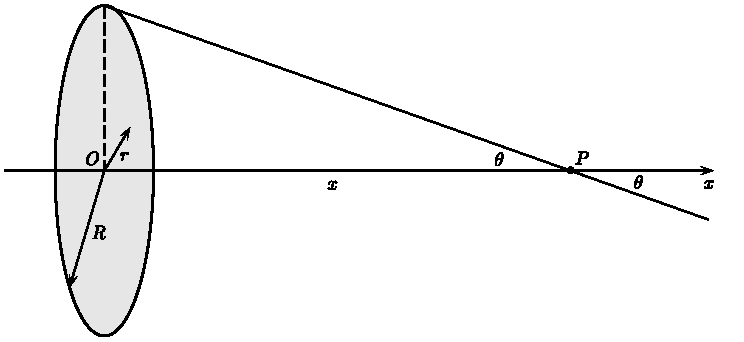
\includegraphics[scale=1.0]{CH09EX03.pdf}}
    \end{figure}
    $$
    \mathrm{d}E=\frac{\sigma \mathrm{d}S}{4\pi\varepsilon_0\left(x^2+r^2\right)}
    $$
    $$
    \cos\theta=\frac{x}{\sqrt{x^2+r^2}}
    $$
    $$
    \sigma=\frac{q}{\pi R^2}
    $$
    
    由于$E_\bot$相互抵消,则$E=E_\parallel$
    $$
    \mathrm{d}E_\parallel=\mathrm{d}E\cdot\cos\theta=\frac{x\sigma\mathrm{d}S}{4\pi\varepsilon_0\left(x^2+r^2\right)^{\frac{3}{2}}}
    $$
    $$
    \mathrm{d}S=\mathrm{d}\left(\pi r^2\right)=2\pi r\mathrm{d}r
    $$
    
    因此
    \begin{eqnarray}
        E=\int\mathrm{d}E_\parallel &=&\int_{0}^{R}\frac{x\sigma}{4\pi\varepsilon_0\left(x^2+r^2\right)^{\frac{3}{2}}}\mathrm{d}S \nonumber \\
        ~&=&\int_{0}^{R}\frac{x\sigma\cdot 2\pi r}{4\pi\varepsilon_0\left(x^2+r^2\right)^{\frac{3}{2}}}\mathrm{d}r \nonumber \\
        ~&=&\frac{x\sigma}{4\varepsilon_0}\int_{0}^{R}\frac{\mathrm{d}r^2}{\left(x^2+r^2\right)^{\frac{3}{2}}} \nonumber \\
        ~&=&\frac{x\sigma}{2\varepsilon_0}\left(\frac{1}{x}-\frac{1}{\sqrt{x^2+R^2}}\right) \nonumber
    \end{eqnarray}
    
    {\sonti 特殊情况}:
    
    当$x\gg R$时
    $$
    E=\frac{q}{4\pi\varepsilon_0x^2}
    $$

    当$x\ll R$时
    $$
    E=\frac{\sigma}{2\varepsilon_0}
    $$
\end{example}
\section{电场线、电场强度通量}
{\sonti 电场线}为假想曲线,曲线上每一点的切线方向都与该点的场强方向一致。其起始于正电荷或无穷远,终止于负电荷或无穷远;任意两条电场线不会相交。电场线越密处,场强越大

{\sonti 电场线数密度}:$\frac{n}{\mathrm{d}S}$

{\sonti 电场强度通量(标量)}:$\varPhi_\mathrm{e}$
\section{高斯定理}
在真空中,通过任一闭合曲面(该闭合曲面称为{\sonti 高斯面})的电场强度通量,等于该曲面内所包围的所有电荷的代数和除以$\varepsilon_0$。\textbf{[这里为了写法简洁清晰,可写为一重积分号]}
$$
\varPhi_\mathrm{e}=\varoiint \boldsymbol{E}\cdot\mathrm{d}\boldsymbol{S}=\oint_S \boldsymbol{E}\cdot\mathrm{d}\boldsymbol{S}=\frac{1}{\varepsilon_0}\sum_{\text{内}}q_i
$$

若高斯面内无点电荷,必有穿入高斯面的电场线数量=穿出高斯面的电场线数量

穿入的电场强度通量是负值,穿出的电场强度通量是正值

电场强度通量$\varPhi$只有面内电荷有关,与面外电荷无关

$E$为高斯面上某点的电场强度,由空间所有电荷产生,与面内外电荷均有关

$\varPhi=0$,不一定面内无电荷,有可能面内电荷等量异号

$\varPhi=0$,不一定高斯面上各点的电场强度均为0

高斯定理说明电场是有源场,也是无旋场

根据闭合曲面法线方向的约定,穿出高斯面的电场强度通量为正,穿入高斯面的电场强度通量为负
\section{静电场的环路定理}
试验电荷$q_0$在静电场中从一点沿任意路径运动到另一点时,静电场力对它所做的功,仅与试验电荷$q_0$及路径的起点和终点位置有关,而与该路径的形状无关

静电力是保守力,静电场是保守场,无旋场。无旋场一定是保守场

{\sonti 静电场的环路定理}:在静电场中,电场强度沿任一闭合路径的线积分为零
$$
\oint \boldsymbol{E}\cdot\mathrm{d}\boldsymbol{l}=0
$$
\section{电势}
{\sonti 电势能}是一个相对的量,需要选择一个零点势能参考点,对于有限带电体,一般选无限远处$E_{\mathrm{p}\infty}=0$
$$
W_{ab}=q_0\int_{a}^{b} \boldsymbol{E}\cdot\mathrm{d}\boldsymbol{l}=-\left(E_{\mathrm{p}b}-E_{\mathrm{p}a}\right)=E_{\mathrm{p}a}-E_{\mathrm{p}b}
$$

试验电荷$q_0$在电场中$a$点的电势能等于将$q_0$由$a$点移至电势能零点时,电场力所做的功

{\sonti 电势(标量)}:
$$
V_a=\frac{E_{\mathrm{p}a}}{q_0}=\int_{a}^{b} \boldsymbol{E}\cdot\mathrm{d}\boldsymbol{l}
$$
单位为$\mathrm{J}\cdot\mathrm{C}^{-1}$,以$\mathrm{V}$表示

对于有限带电体,通常取无穷远处电势为零,则
$$
V_a=\frac{E_{\mathrm{p}a}}{q_0}=\int_{a}^{\infty} \boldsymbol{E}\cdot\mathrm{d}\boldsymbol{l}
$$

{\sonti 电势差}:$V_a-V_b$为$a$、$b$两点的电势差,以$U_{ab}$表示,有
$$
U_{ab}=V_a-V_b=\int_{a}^{\infty} \boldsymbol{E}\cdot\mathrm{d}\boldsymbol{l}-\int_{b}^{\infty} \boldsymbol{E}\cdot\mathrm{d}\boldsymbol{l}=\int_{a}^{b} \boldsymbol{E}\cdot\mathrm{d}\boldsymbol{l}
$$
$$
W_{ab}=q_0U_{ab}=q_0\left(V_a-V_b\right)
$$

{\sonti 点电荷电场电势分布}:
$$
V_A=\int_{A}^{\infty} \boldsymbol{E}\cdot\mathrm{d}\boldsymbol{l}=\int_{A}^{\infty}\frac{q}{4\pi\varepsilon_0r^2}\boldsymbol{e}_r\cdot\mathrm{d}\boldsymbol{r}=\int_{A}^{\infty}\frac{q}{4\pi\varepsilon_0r^2}\mathrm{d}r=\frac{q}{4\pi\varepsilon_0r}
$$

{\sonti 连续带电体的电势}:
$$
\mathrm{d}V=\frac{\mathrm{d}q}{4\pi\varepsilon_0r}
$$
$$
V=\int\mathrm{d}V=\int\frac{\mathrm{d}q}{4\pi\varepsilon_0r}
$$
\begin{example}
    一均匀带电圆环,半径为$R$,电荷量为$q$,求其轴线上任一点电势。
    
    \noindent\textbf{解}
    \begin{figure}[H]
        \centerline{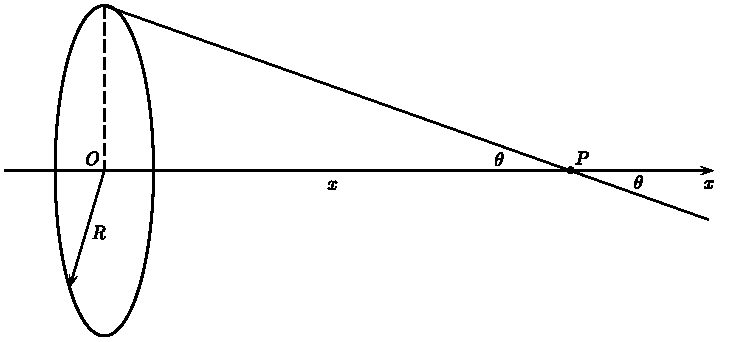
\includegraphics[scale=1.0]{CH09EX04.pdf}}
    \end{figure}
    $$
    E=\frac{qx}{4\pi\varepsilon_0\left(x^2+R^2\right)^{\frac{3}{2}}}
    $$
    \begin{eqnarray}
    V_P &=&\int_{x}^{\infty}\frac{qx}{4\pi\varepsilon_0\left(x^2+R^2\right)^{\frac{3}{2}}}\mathrm{d}x \nonumber \\
    ~&=&\frac{q}{8\pi\varepsilon_0}\int_{x}^{\infty}\frac{\mathrm{d}\left(x^2+R^2\right)}{\left(x^2+R^2\right)^{\frac{3}{2}}} \nonumber \\
    ~&=&\frac{q}{4\pi\varepsilon_0\sqrt{x^2+R^2}} \nonumber
    \end{eqnarray}
    \noindent\textbf{另解}
    $$
    V_P=\int\mathrm{d}V_P
    $$
    $$
    \mathrm{d}V_P=\frac{\mathrm{d}q}{4\pi\varepsilon_0r}=\frac{\mathrm{d}q}{4\pi\varepsilon_0\sqrt{x^2+R^2}}
    $$
    $$
    V_P=\int\mathrm{d}V_P=\int_q\frac{\mathrm{d}q}{4\pi\varepsilon_0\sqrt{x^2+R^2}}=\frac{q}{4\pi\varepsilon_0\sqrt{x^2+R^2}}
    $$
\end{example}
\begin{example}
    一均匀带电球体,电荷体密度为$\rho$,半径为$R$,求球体内外任一点的电势。

    \noindent\textbf{解}
    \begin{figure}[H]
        \centerline{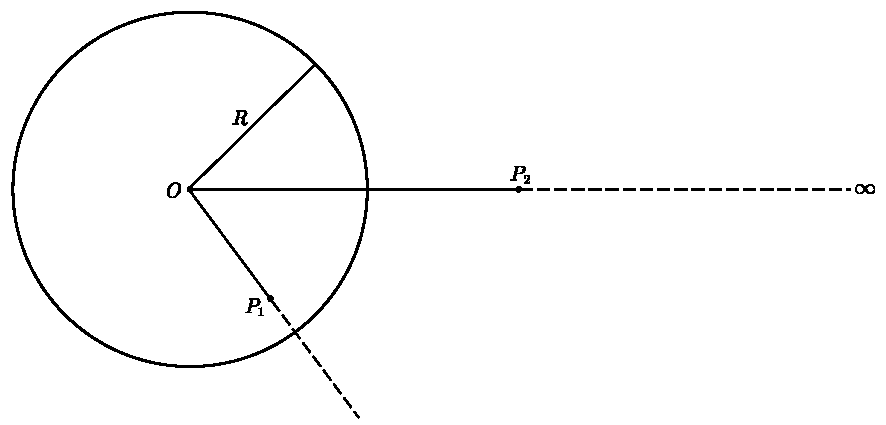
\includegraphics[scale=0.8]{CH09EX05.pdf}}
    \end{figure}
    {\sonti 首先计算电场分布}:
    \begin{itemize}
        \item $r<R$时
        $$
        \oint_S \boldsymbol{E_1}\cdot\mathrm{d}\boldsymbol{S}=\oint_S E_1\mathrm{d}S\cdot\cos\theta,\cos\theta=1
        $$
        $$
        E_1\oint_S\mathrm{d}S=\frac{1}{\varepsilon_0}\sum_{\text{内}}q_i
        $$
        因此
        $$
        4\pi r^2\mathrm{d}E_1=\frac{\mathrm{d}q}{\varepsilon_0} \Rightarrow 4\pi r^2\int\mathrm{d}E_1=\frac{1}{\varepsilon_0}\int\mathrm{d}q
        $$
        又
        $$
        \mathrm{d}q=\rho\mathrm{d}V
        $$
        $$
        \mathrm{d}V=\mathrm{d}\left(\frac{4}{3}\pi r^3\right)=4\pi r^2\mathrm{d}r
        $$
        所以有
        $$
        4\pi r^2E_1=\frac{1}{\varepsilon_0}\int\rho\cdot4\pi r^2\mathrm{d}r
        $$
        因此
        $$
        E_1=\frac{\rho r}{3\varepsilon_0}
        $$
        \item $r>R$时
        $$
        \mathrm{d}q=\rho\mathrm{d}V=\rho\mathrm{d}\left(\frac{4}{3}\pi R^3\right)=\rho\cdot4\pi R^2\mathrm{d}R
        $$
        又
        $$
        4\pi r^2E_2=\frac{1}{\varepsilon_0}\int\rho\cdot4\pi R^2\mathrm{d}R
        $$
        因此
        $$
        E_2=\frac{\rho R^3}{3\varepsilon_0r^2}
        $$
    \end{itemize}
    
    因此,场强分布为
    $$
    E=\left\{ \begin{array}{l}
        \frac{\rho r}{3\varepsilon_0},r<R\\
        \frac{\rho R^3}{3\varepsilon_0r^2},r>R\\
    \end{array} \right. 
    $$

    {\sonti 再计算电势分布}:
    \begin{itemize}
        \item 当$r>R$时,设球面外离球心为$r$的$P_2$处的电势为$V_2$,则有
        $$
        V_2=\int_{r}^{\infty}E_2\mathrm{d}r=\int_{r}^{\infty}\frac{\rho R^3}{3\varepsilon_0r^2}\mathrm{d}r=\frac{\rho R^3}{3\varepsilon_0r}
        $$
        \item 当$r<R$时,设球面内离球心为$r$的$P_1$处的电势为$V_1$,则有
        $$
        V_1=\int_{r}^{R}E_1\mathrm{d}r+\int_{R}^{\infty}E_2\mathrm{d}r=\int_{r}^{R}\frac{\rho r}{3\varepsilon_0}\mathrm{d}r+\int_{R}^{\infty}\frac{\rho R^3}{3\varepsilon_0r^2}\mathrm{d}r=\frac{\rho}{6\varepsilon_0}\left(3R^2-r^2\right)
        $$
    \end{itemize}
    
    因此,电势分布为
    $$
    V=\left\{ \begin{array}{l}
        \frac{\rho}{6\varepsilon_0}\left(3R^2-r^2\right),r<R\\
        \frac{\rho R^3}{3\varepsilon_0r},r>R\\
    \end{array} \right. 
    $$
\end{example}
\section{等势面}
{\sonti 等势面}:电场中电势相等的点组成的曲面

电荷沿等势面运动时,电场力不做功,即$q\boldsymbol{E}\cdot\mathrm{d}\boldsymbol{l}=0 \Rightarrow \boldsymbol{E}\cdot\mathrm{d}\boldsymbol{l}=0$,因此$\boldsymbol{E}$与$\mathrm{d}\boldsymbol{l}$垂直,则等势面处处与电场线垂直
\section{电场中的导体}
{\sonti 导体的静电平衡状态}:起初附加电场$\boldsymbol{E'}$与外电场$\boldsymbol{E}_0$反向,且$\boldsymbol{E'}<\boldsymbol{E}_0$,逐渐$\boldsymbol{E'}=\boldsymbol{E}_0$,此时导体内部场强$E=0$,导体表面电荷分布稳定

{\sonti 静电感应现象}:在外电场作用下,引起导体中电荷重新分布而呈现的带电现象

当导体内没有电荷作定向移动时,导体处于静电平衡状态

导体平衡后,导体内部以及导体表面无电荷作定向运动,此时导体表面电场强度方向与表面垂直

导体处于静电平衡状态时,必须满足:
\begin{itemize}
    \item 导体内部电场强度处处为零
    \item 导体表面上的电场强度处处垂直于导体表面
\end{itemize}

处于静电平衡状态的导体具备以下的性质:
\begin{itemize}
    \item 整个导体是等势体,导体表面是等势面,$U_{ab}=\int_{a}^{b}\boldsymbol{E}\cdot\mathrm{d}\boldsymbol{l}=0$
    \item 导体内部不存在净电荷,电荷均分布在导体的表面上
\end{itemize}

\textbf{曲率与曲率半径呈倒数关系}

曲率越大(弯曲程度越大)处,即尖端部分,表面电荷面密度越大;曲率越小处,表面电荷面密度越小。表面凹处,曲率为负,电荷面密度更小

防止尖端放电,高压设备的电极做成光滑的球形。避雷针利用尖端放电原理

对于腔内没有带电体的空腔导体,导体空腔内表面上的电荷代数和为零

腔内没有电荷的导体空腔在静电平衡时,其内表面没有电荷分布,空腔内没有电场,电势处处相等且等于导体的电势

腔内有带电体的空腔导体,空腔内表面必定带有与腔内带电体等量异号的电荷。其带电情况如\textcolor{blue}{\cref{fig:空腔导体内有带电体带电情况}}所示
\begin{figure}[H]
    \centerline{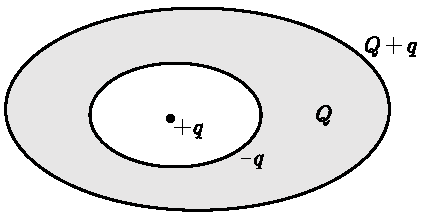
\includegraphics[scale=1.0]{空腔导体内有带电体带电情况.pdf}}
    \caption{空腔导体内有带电体带电情况}\label{fig:空腔导体内有带电体带电情况}
\end{figure}
{\sonti 静电屏蔽}:只要处于静电平衡,腔内必定不存在电场。金属导体对于放在它的空腔内的物体有保护作用,使物体不受外电场的影响
\section{电容、电容器}
{\sonti 孤立导体(实际上不存在)}周围没有其他带电体和导体

设一孤立导体带电荷量为$q$,且有一定电势$V$,则孤立导体的电容为
$$
C=\frac{q}{V}
$$

若在真空中,有一半径为$R$,带电为$q$的孤立导体球,选取无穷远为电势零点,则其电容为
$$
C=\frac{q}{V}=\frac{q}{\frac{q}{4\pi\varepsilon_0R}}=4\pi\varepsilon_0R
$$

孤立导体的电容只与导体自身形状、大小、周围介质有关。它反映了孤立导体储存电荷和电能的能力

{\sonti 电容单位}:$\mathrm{F}$,$1\mathrm{F}=10^6\,\upmu\mathrm{F}=10^{12}\,\mathrm{pF}$

{\sonti 电容器及其电容}:
$$
C=\frac{q}{V_1-V_2}=\frac{q}{U}
$$
\begin{itemize}
    \item {\sonti 平行板电容器}:设$A$、$B$两板平行,面积均为$S$,距离为$d$,带电荷量分别为$+q$、$-q$,极板线度远大于$d$,且不计边缘效应。将两板间电场视为均匀电场,如\textcolor{blue}{\cref{fig:平行板电容器}}所示
    \begin{figure}[H]
        \centerline{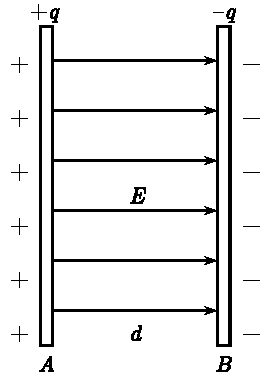
\includegraphics[scale=0.8]{平行板电容器.pdf}}
        \caption{平行板电容器}\label{fig:平行板电容器}
    \end{figure}
    则场强大小为
    $$
    E=2\times\frac{\sigma}{2\varepsilon_0}=\frac{\sigma}{\varepsilon_0}=\frac{q}{\varepsilon_0S}
    $$
    则两板之间电势差为
    $$
    U_{AB}=Ed=\frac{qd}{\varepsilon_0S}
    $$
    则真空平行板电容器电容为
    $$
    C=\frac{q}{U_{AB}}=\frac{q}{\frac{qd}{\varepsilon_0S}}=\frac{\varepsilon_0S}{d}
    $$
    \item {\sonti 球形电容器}:设内、外球壳的半径分别为$R_A$,$R_B$,内球壳带电荷量为$+q$,外球壳带电荷量为$-q$,如\textcolor{blue}{\cref{fig:球形电容器}}所示
    \begin{figure}[H]
        \centerline{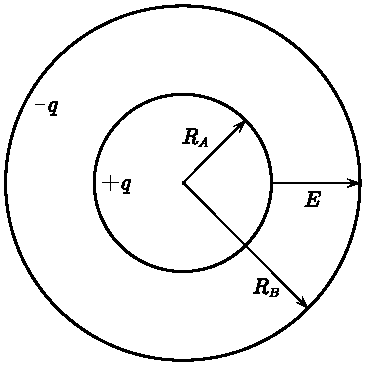
\includegraphics[scale=0.8]{球形电容器.pdf}}
        \caption{球形电容器}\label{fig:球形电容器}
    \end{figure}
    在两球壳之间,即$R_A<r<R_B$,由高斯定理,有
    $$
    4\pi r^2E=\frac{+q}{\varepsilon_0}
    $$
    因此
    $$
    E=\frac{q}{4\pi\varepsilon_0r^2},R_A<r<R_B
    $$
    则两球壳之间电势差为
    $$
    U_{AB}=\int_{A}^{B}\boldsymbol{E}\cdot\mathrm{d}\boldsymbol{l}=\int_{R_A}^{R_B}\frac{q}{4\pi\varepsilon_0r^2}\mathrm{d}r=\frac{q}{4\pi\varepsilon_0}\left(\frac{1}{R_A}-\frac{1}{R_B}\right)
    $$
    则同心球形电容器电容为
    $$
    C=\frac{q}{U_{AB}}=\frac{q}{\frac{q}{4\pi\varepsilon_0}\left(\frac{1}{R_A}-\frac{1}{R_B}\right)}=\frac{4\pi\varepsilon_0R_AR_B}{R_B-R_A}
    $$
    \item {\sonti 圆柱形电容器}:设两柱面半径分别为$R_A$,$R_B$,所带电荷量分别为$+q$,$-q$,圆柱高为$l$,除边缘外,电荷均匀分布在内、外两圆柱面上,如\textcolor{blue}{\cref{fig:圆柱形电容器}}所示
    \begin{figure}[H]
        \centerline{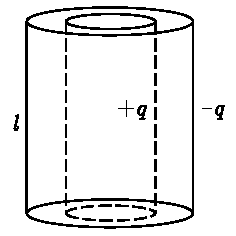
\includegraphics[scale=1.4]{圆柱形电容器.pdf}}
        \caption{圆柱形电容器}\label{fig:圆柱形电容器}
    \end{figure}
    $$
    +q=\sigma S=\sigma\cdot2\pi R_Al=\sigma\cdot2\pi R_Al
    $$
    在两圆柱面之间,即$R_A<r<R_B$,由高斯定理,有
    $$
    2\pi rlE=\frac{\sigma\cdot2\pi R_Al}{\varepsilon_0}
    $$
    因此
    $$
    E=\frac{\sigma R_A}{\varepsilon_0r}
    $$
    则两圆柱面之间电势差为
    $$
    U_{AB}=\int_{A}^{B}\boldsymbol{E}\cdot\mathrm{d}\boldsymbol{l}=\int_{R_A}^{R_B}\frac{\sigma R_A}{\varepsilon_0r}\mathrm{d}r=\frac{\sigma R_A}{\varepsilon_0}\left(\ln R_B-\ln R_A\right)
    $$
    则圆柱形电容器电容为
    $$
    C=\frac{q}{U_{AB}}=\frac{\sigma\cdot2\pi R_Al}{\frac{\sigma R_A}{\varepsilon_0}\left(\ln R_B-\ln R_A\right)}=\frac{2\pi\varepsilon_0l}{\ln R_B-\ln R_A}
    $$
\end{itemize}
\section{静电场中的电介质}
{\sonti 电介质中的电场}

当电介质受到外电场$\boldsymbol{E}_0$作用而极化时,电介质端面出现极化电荷,计划电荷也会产生电场,为$\boldsymbol{E}'$。因此,电介质中的电场$\boldsymbol{E}$是外电场$\boldsymbol{E}_0$与电介质中的电场$\boldsymbol{E}'$的矢量和,即
$$
\boldsymbol{E}=\boldsymbol{E}_0+\boldsymbol{E}'
$$
而又由于$\boldsymbol{E}'$与$\boldsymbol{E}_0$的反向,因此介质中电场强度的大小为
$$
E=E_0-E'
$$

设充满均匀且各向同性介质的平行板电容器两极板上自由电荷面密度为$\pm\sigma_0$,介质端面极化电荷面密度为$\pm\sigma'$,如\textcolor{blue}{\cref{fig:电介质中的电场}}所示
\begin{figure}[H]
    \centerline{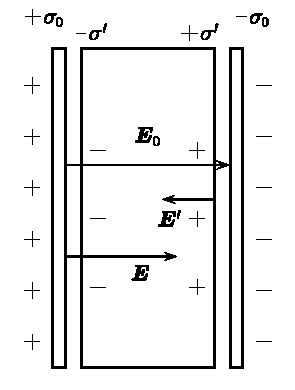
\includegraphics[scale=1.0]{电介质中的电场.pdf}}
    \caption{电介质中的电场}\label{fig:电介质中的电场}
\end{figure}
$$
E_0=\frac{\sigma_0}{\varepsilon_0},E'=\frac{\sigma'}{\varepsilon_0}
$$
$$
E=E_0-E'=\frac{\sigma_0-\sigma'}{\varepsilon_0}
$$
因此,电介质中的场强总是小于真空中的场强。

两板之间的电场强度$\boldsymbol{E}$的值仅为真空时两板之间电场强度$\boldsymbol{E_0}$值的$\frac{1}{\varepsilon_{\mathrm{r}}}$倍,即
$$
E=\frac{E_0}{\varepsilon_{\mathrm{r}}},\varepsilon_{\mathrm{r}}>1
$$

{\sonti 相对电容率(无量纲)}:$\varepsilon_{\mathrm{r}}$

极化电荷与自由电荷的关系为
$$
\sigma'=\sigma_0\left(1-\frac{1}{\varepsilon_{\mathrm{r}}}\right)
$$

{\sonti 电介质中的高斯定理}:

设平行板电容器两极板上自由电荷面密度为$\pm\sigma_0$,两板之间充满相对电容率为$\varepsilon_{\mathrm{r}}$的各向同性电介质,电介质极化后端面出现极化电荷面密度为$\pm\sigma'$,作一底面积为$\Delta$的圆柱形高斯面,两底分别在电介质和导体板中,侧面与导体板垂直,如\textcolor{blue}{\cref{fig:电介质中的高斯定理}}所示。
\begin{figure}[H]
    \centerline{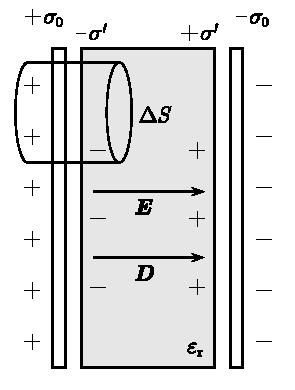
\includegraphics[scale=1.0]{电介质中的高斯定理.pdf}}
    \caption{电介质中的高斯定理}\label{fig:电介质中的高斯定理}
\end{figure}
由高斯定理,有
$$
\oint_S \boldsymbol{E}\cdot\mathrm{d}\boldsymbol{S}=\frac{1}{\varepsilon_0}\sum_{S\text{内}}\left(q_0+q'\right)=\frac{1}{\varepsilon_0}\left(\sigma_0-\sigma'\right)\Delta S
$$

由于
$$
\sigma'=\sigma_0\left(1-\frac{1}{\varepsilon_{\mathrm{r}}}\right)
$$

则可得
$$
\oint_S \boldsymbol{E}\cdot\mathrm{d}\boldsymbol{S}=\frac{\sigma_0}{\varepsilon_0\varepsilon_{\mathrm{r}}}\Delta S=\frac{q_0}{\varepsilon}
$$
其中$\varepsilon=\varepsilon_0\varepsilon_{\mathrm{r}}$为电介质的电容率

还可得到
$$
\oint_S \varepsilon\boldsymbol{E}\cdot\mathrm{d}\boldsymbol{S}=q_0
$$
记$\boldsymbol{D}=\varepsilon\boldsymbol{E}$为电位移,其单位为$\mathrm{C}\cdot\mathrm{m}^{-2}$,于是得
$$
\oint_S \boldsymbol{D}\cdot\mathrm{d}\boldsymbol{S}=q_0
$$

上式即为\textbf{电介质中的高斯定理},它表示:通过电介质中任一闭合曲面的电位移通量,等于该曲面内所包围的自由电荷的代数和

{\sonti 电介质中静电场的计算}
\begin{example}
    在半径为$R$的金属球外,有一外半径为$R'$的同心均匀电介质层,其相对电容率为$\varepsilon_{\mathrm{r}}$,金属球电荷量为$Q$,求场强及电势的空间分布。
    \begin{figure}[H]
        \centerline{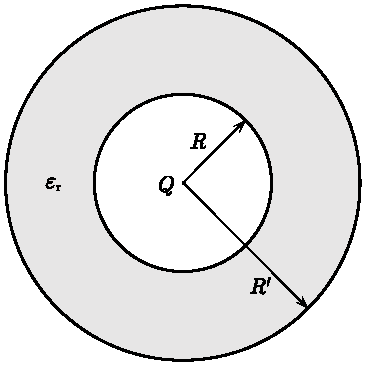
\includegraphics[scale=1.0]{CH09EX06.pdf}}
    \end{figure}
    \noindent\textbf{解}

    {\sonti 场强的空间分布}:
    
    由介质中的高斯定理
    $$
    \oint_S \boldsymbol{D}\cdot\mathrm{d}\boldsymbol{S}=\sum_{S\text{内}}q_0
    $$
    
    可得
    $$
    D\cdot 4\pi r^2=\left\{ \begin{array}{l}
        0,r<R\\
        Q,r>R\\
    \end{array} \right. 
    $$
    
    由$E=\frac{D}{\varepsilon}$,可得到
    $$
    E=\left\{ \begin{array}{l}
        0,r<R\\
        \frac{Q}{4\pi r^2\varepsilon _0\varepsilon _{\text{r}}},R<r<R'\\
        \frac{Q}{4\pi r^2\varepsilon _0},r>R'\\
    \end{array} \right. 
    $$
    
    {\sonti 电势的空间分布}:
    \begin{itemize}
        \item 当$r>R'$时,设介质外离球心为$r$处的电势为$V_3$,则有
        $$
        V_3=\int_{r}^{\infty}\boldsymbol{E}\cdot\mathrm{d}\boldsymbol{r}=\int_{r}^{\infty}\frac{Q}{4\pi r^2\varepsilon _0}\mathrm{d}r=\frac{Q}{4\pi\varepsilon_0r}
        $$
        \item 当$R<r<R'$时,设介质层中离球心为$r$处的电势为$V_2$,则有
        \begin{eqnarray}
            V_2=\int_{r}^{R'}\boldsymbol{E}\cdot\mathrm{d}\boldsymbol{r}+\int_{R'}^{\infty}\boldsymbol{E}\cdot\mathrm{d}\boldsymbol{r} &=& \int_{r}^{R'}\frac{Q}{4\pi r^2\varepsilon _0\varepsilon _{\text{r}}}\mathrm{d}r+\int_{R'}^{\infty}\frac{Q}{4\pi r^2\varepsilon _0}\mathrm{d}r \nonumber \\
            ~&=& \frac{Q}{4\pi\varepsilon_0}\left[\frac{1}{\varepsilon_{\mathrm{r}}}\left(\frac{1}{r}-\frac{1}{R'}\right)+\frac{1}{R'}\right] \nonumber
        \end{eqnarray}
        \item 当$r=R$时,设金属球的电势为$V_1$,则有
        \begin{eqnarray}
            V_1=\int_{R}^{R'}\boldsymbol{E}\cdot\mathrm{d}\boldsymbol{r}+\int_{R'}^{\infty}\boldsymbol{E}\cdot\mathrm{d}\boldsymbol{r} &=& \int_{R}^{R'}\frac{Q}{4\pi r^2\varepsilon _0\varepsilon _{\text{r}}}\mathrm{d}r+\int_{R'}^{\infty}\frac{Q}{4\pi r^2\varepsilon _0}\mathrm{d}r \nonumber \\
            ~&=& \frac{Q}{4\pi\varepsilon_0}\left[\frac{1}{\varepsilon_{\mathrm{r}}}\left(\frac{1}{R}-\frac{1}{R'}\right)+\frac{1}{R'}\right] \nonumber
        \end{eqnarray}
    \end{itemize}
\end{example}
\section{静电场的能量}
{\sonti 电容器所贮存的电能}:
$$
W_e=\frac{1}{2}CU^2
$$
由$C=\frac{Q}{U}$,可以得到
$$
W_e=\frac{Q^2}{2C}=\frac{1}{2}QU
$$

对于一般的静电场,电场能量为
$$
W_e=\frac{1}{2}\varepsilon E^2 Sd=\frac{1}{2}\varepsilon E^2 V
$$

{\sonti 电场能量密度}:
$$
w_e=\frac{W_e}{V}=\frac{1}{2}\varepsilon E^2
$$

对于非均匀电场,电场能量密度是随着场强变化的,电场总能量是电场能量密度的体积分,即
$$
W_e=\int_V w_e\mathrm{d}V=\int_V \frac{1}{2}\varepsilon E^2\mathrm{d}V
$$
\chapter{恒定磁场}
\newpage
\section{磁场}
{\sonti 奥斯特实验}:奥斯特发现通电直导线附近的小磁针会发生偏转,其表明电流可以对磁铁施加作用力

{\sonti 磁感应强度}:
\begin{itemize}
    \item 方向:将小磁针$\mathrm{N}$极所指的方向规定为磁场中该点的磁感应强度$\boldsymbol{B}$的方向
    \item 大小:当运动试验电荷$q$垂直于该特定方向运动时,该电荷受到磁场力最大,记为$F_\mathrm{max}$,则有
    $$
    B=\frac{F_\mathrm{max}}{qv}
    $$
    \item 单位:$\mathrm{T}$,$1\,\mathrm{T}=1\,\mathrm{N}\cdot\mathrm{A}^{-1}\cdot\mathrm{m}^{-1}$
\end{itemize}
\section{毕奥-萨伐尔定律}
{\sonti 毕奥-萨伐尔定律}:

在真空中,电流元$I\mathrm{d}\boldsymbol{l}$在空间任意点$P$处所产生的磁场为
$$
\mathrm{d}\boldsymbol{B}=\frac{\mu_0}{4\pi}\frac{I\mathrm{d}\boldsymbol{l}\times\boldsymbol{e}_r}{r^2}
$$
大小为
$$
\mathrm{d}B=\frac{\mu_0}{4\pi}\frac{I\mathrm{d}l\cdot\sin\theta}{r^2}
$$
其中$\theta$为$I\mathrm{d}\boldsymbol{l}$与$\boldsymbol{e}_r$的夹角,$\mathrm{B}$的方向由$I\mathrm{d}\boldsymbol{l}$与$\boldsymbol{e}_r$的矢量叉乘确定,可见$\mathrm{d}B$垂直于$I\mathrm{d}\boldsymbol{l}$与$\boldsymbol{e}_r$所决定的平面;$\mu_0$为真空磁导率,其值为
$$
\mu_0=4\pi\times10^{-7}\,\mathrm{N}\cdot\mathrm{A}^{-2}
$$
因此有
$$
\frac{\mu_0}{4\pi}=10^{-7}\,\mathrm{N}\cdot\mathrm{A}^{-2}
$$

由于磁感应强度$\boldsymbol{B}$遵从磁场的叠加原理,因此有
$$
\boldsymbol{B}=\int\mathrm{d}\boldsymbol{B}=\int\frac{\mu_0}{4\pi}\frac{I\mathrm{d}\boldsymbol{l}\times\boldsymbol{e}_r}{r^2}
$$

{\sonti 运动电荷的磁场}:

设电流元$I\mathrm{d}\boldsymbol{l}$的横截面面积为$S$,载流子(正电荷)的电荷量为$q$,单位体积内有$n$个做定向运动的载流子,它们速度运动均为矢量$\boldsymbol{v}$,则单位时间内通过横截面$S$的电荷量为$qnvS$,及电流强度为$I=qnvS$,电流元中共有$N=nS\mathrm{d}l$个载流子,且忽略电流元内各载流子到$P$点矢径$r$的差异,则每个运动载流子在$P$点激发的磁场为
$$
\boldsymbol{B}=\frac{\mathrm{d}\boldsymbol{B}}{N}=\frac{1}{nS\mathrm{d}l}\frac{\mu_0}{4\pi}\frac{qnS\mathrm{d}l\boldsymbol{v}\times\boldsymbol{e}_r}{r^2}
$$
即有
$$
\boldsymbol{B}=\frac{\mu_0}{4\pi}\frac{q\boldsymbol{v}\times\boldsymbol{e}_r}{r^2}
$$

{\sonti 电流产生的磁场大小结论}:
\begin{itemize}
    \item \textbf{载流直导线的磁场}:设载流直导线长为$L$,通有电流$I$,导线旁任意一点$P$与导线的距离为$r$,如\textcolor{blue}{\cref{fig:载流直导线的磁场}}所示,则$P$处的磁感应强度大小为
    $$
    B=\frac{\mu_0I}{2\pi r}\left(\cos\theta_1-\cos\theta_2\right)
    $$
    \begin{figure}[H]
        \centerline{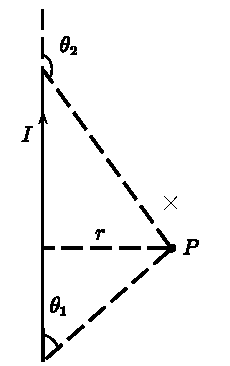
\includegraphics[scale=1.0]{载流直导线的磁场.pdf}}
        \caption{载流直导线的磁场}
        \label{fig:载流直导线的磁场}
    \end{figure}
    若载流直导线无限长,则此时有$\theta_1=0$,$\theta_2=\pi$,则$P$处的磁感应强度大小为
    $$
    B=\frac{\mu_0I}{2\pi r}
    $$
    \item \textbf{载流圆线圈轴线上的磁场}:设载流圆线圈半径为$R$,通有电流$I$,$P$点为其轴线上任意一点,它与圆心距离为$x$,如\textcolor{blue}{\cref{fig:载流圆线圈轴线上的磁场}}所示,则$P$处的磁感应强度大小为
    $$
    B=\frac{\mu_0I R^2}{2\left(R^2+x^2\right)^{\frac{3}{2}}}
    $$
    \begin{figure}[H]
        \centerline{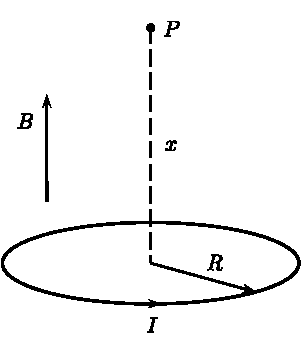
\includegraphics[scale=0.88]{载流圆线圈轴线上的磁场.pdf}}
        \caption{载流圆线圈轴线上的磁场}
        \label{fig:载流圆线圈轴线上的磁场}
    \end{figure}
    当$x=0$时,在线圈中线点$O$的磁感应强度大小为
    $$
    B=\frac{\mu_0 I}{2R}
    $$
    一般地,一段圆弧在圆心处的磁感应强度大小为
    $$
    B=\frac{\mu_0 I}{2r}\frac{\varphi}{2\pi}
    $$
    其中$\varphi$为圆弧的弧度制角度
    \item \textbf{载流直螺线管轴线上的磁场}:设螺线管长为$L$,半径为$R$,线圈是密绕的,总匝数为$N$,则定义匝密度为$n=\frac{N}{L}$,即单位长度上绕有$n$匝线圈,同时通有电流$I$,$P$点为其轴线上任意一点,如\textcolor{blue}{\cref{fig:载流直螺线管轴线上的磁场}}所示,则$P$处的磁感应强度大小为
    $$
    B=\frac{\mu_0nI}{2}\left(\cos\beta_1-\cos\beta_2\right)
    $$
    \begin{figure}[H]
        \centerline{\includegraphics[scale=1.0]{载流直螺线管轴线上的磁场.pdf}}
        \caption{载流直螺线管轴线上的磁场}
        \label{fig:载流直螺线管轴线上的磁场}
    \end{figure}
    若载流直螺线管无限长,则此时有$\beta_1=0$,$\beta_2=\pi$,则轴线上磁感应强度大小为
    $$
    B=\mu_0nI
    $$
    若载流直螺线管半无限长,则有$\beta_1=0$,$\beta_2=\frac{\pi}{2}$或$\beta_1=\frac{\pi}{2}$,$\beta_2=\pi$,则轴线上磁感应强度大小为
    $$
    B=\frac{1}{2}\mu_0nI
    $$
\end{itemize}
\begin{example}
    一根载流导线弯成如图平面曲线,其拐弯部分为半圆形,两直线平行并分别在$a$,$b$两点与半圆相切,已知导线中电流强度为$I$,且流向在图中已标出,圆半径为$R$,直线部分长度远大于$R$,求圆心$O$处的磁感应强度。
    \begin{figure}[H]
        \centerline{\includegraphics[scale=0.88]{CH10EX01.pdf}}
    \end{figure}

    \noindent\textbf{解}
    \begin{eqnarray}
        B &=&B_1+B_2+B_3 \nonumber \\
        ~&=& \frac{\mu_0I}{4\pi R}\left(\cos0-\cos\frac{\pi}{2}\right)+\frac{\mu_0I}{4\pi R}\left(\cos\frac{\pi}{2}-\cos\pi\right)+\frac{1}{2}\cdot\frac{\mu_0I}{2R} \nonumber \\
        ~&=&\frac{\mu_0I}{2\pi R}+\frac{\mu_0I}{4R} \nonumber
    \end{eqnarray}

    磁感应强度的方向为垂直于纸平面向内
\end{example}
\section{磁通量}
{\sonti 磁感线}:

磁感应线是一些有方向的曲线,磁感应线上任一点的切线方向与该电磁感应强度的方向相同;磁感应线的密度,即通过磁场中某地点处垂直于磁场方向的单位面积的磁感应线数目,等于该电磁感应强度的大
小。因此,磁场较强的地方,磁感线较密集,反之,磁感线较稀疏

{\sonti 磁通量}:

通过某一曲面的磁感线数目称为通过该曲面的磁通量,用$\varPhi_\mathrm{m}$表示
$$
\varPhi_\mathrm{m}=\int_S \boldsymbol{B}\cdot\mathrm{d}\boldsymbol{S}
$$
单位为$\mathrm{Wb}$,$1\,\mathrm{Wb}=1\,\mathrm{T}\cdot\mathrm{m}^2$
\section{磁场的高斯定理}
通过任意闭合曲面的磁通量必为零,即
$$
\oint_S\boldsymbol{B}\cdot\mathrm{d}\boldsymbol{S}=0
$$

静电场是有源场,而磁场是无源场、有旋场

\begin{example}
    一矩形导线框与一长直载流导线共面,如下图所示,求通过矩形线框所围面积的磁通量$\varPhi_\mathrm{m}$。
    \begin{figure}[H]
        \centerline{\includegraphics[scale=0.88]{CH10EX02.pdf}}
    \end{figure}

    \noindent\textbf{解}

    无限长直导线的磁场分布为
    $$
    B=\frac{\mu_0I}{2\pi r}
    $$

    又
    $$
    \mathrm{d}S=l_1\mathrm{d}r
    $$

    则
    $$
    \mathrm{d}\varPhi_\mathrm{m}=\boldsymbol{B}\cdot\mathrm{d}\boldsymbol{S}=B\mathrm{d}S=\frac{\mu_0Il_1}{2\pi r}\mathrm{d}r
    $$

    因此
    \begin{eqnarray}
        \varPhi_\mathrm{m} &=&\int_S\mathrm{d}\varPhi_\mathrm{m} \nonumber \\
        ~&=&\int_{h}^{h+l_2}\frac{\mu_0Il_1}{2\pi r}\mathrm{d}r \nonumber \\
        ~&=&\frac{\mu_0 Il_1}{2\pi}\ln\frac{h+l_2}{h} \nonumber
    \end{eqnarray}
\end{example}
\section{安培环路定理}
在真空的恒定磁场中,磁感应强度$\boldsymbol{B}$沿任意闭合回路$l$的线积分(环流),等于该闭合路径所围住的电流强度的代数和的$\mu_0$倍,即
$$
\oint_l\boldsymbol{B}\cdot\mathrm{d}\boldsymbol{l}=\mu_0\sum_{i=1}^nI_i
$$

若有多根直载流导线穿过闭合路径$l$,上式同样成立;上式右端的$\sum\limits_{i=1}^{n}I_i$只包括闭合路径$l$围住的电流

$\boldsymbol{B}$为环路上一点的磁感应强度,不是任意点的,其与环路内外电流均有关

若$\oint_l\boldsymbol{B}\cdot\mathrm{d}\boldsymbol{l}=0$,并不一定能说明环路上各点的$B=0$,也不能说明环路内无电流

静电场是保守场,磁场是涡旋场
\begin{example}
    如下图所示,当只有电流$I_1$时,计算$\boldsymbol{B}$沿回路$\boldsymbol{l}$的环流。之后依次加入电流$I_2$,$I_3$,$I_4$再分别计算$\boldsymbol{B}$沿回路$\boldsymbol{l}$的环流。
    \begin{figure}[H]
        \centerline{\includegraphics[scale=0.88]{CH10EX03.pdf}}
    \end{figure}

    \noindent\textbf{解}

    仅有电流$I_1$穿过回路时,由右手螺旋关系可以确定$I_1$取正向,因此环流
    $$
    \oint_l\boldsymbol{B}\cdot\mathrm{d}\boldsymbol{l}=\mu_0I_1
    $$

    当电流$I_1$,$I_2$穿过回路时,有
    $$
    \oint_l\boldsymbol{B}\cdot\mathrm{d}\boldsymbol{l}=\mu_0(I_1+2I_2)
    $$

    当电流$I_1$,$I_2$,$I_3$穿过回路时,有
    $$
    \oint_l\boldsymbol{B}\cdot\mathrm{d}\boldsymbol{l}=\mu_0(I_1+2I_2+0)=\mu_0(I_1+2I_2)
    $$

    当电流$I_1$,$I_2$,$I_3$,$I_4$穿过回路时,有
    $$
    \oint_l\boldsymbol{B}\cdot\mathrm{d}\boldsymbol{l}=\mu_0(I_1+2I_2-I_4)
    $$
\end{example}
\begin{example}
    设一无限长载流圆柱面半径为$R$,通有电流$I$,求其内外的磁场分布。
    \begin{figure}[H]
        \centerline{\includegraphics[scale=0.88]{CH10EX04.pdf}}
    \end{figure}
    \noindent\textbf{解}

    当$0<r<R$时,有
    $$
    \oint_l\boldsymbol{B}\cdot\mathrm{d}\boldsymbol{l}=0
    $$

    则
    $$
    B=0
    $$
    
    当$r>R$时,有
    $$
    \oint_l\boldsymbol{B}\cdot\mathrm{d}\boldsymbol{l}=\mu_0I
    $$

    则
    $$
    B=\frac{\mu_0I}{2\pi r}
    $$

    因此,该无限长载流圆柱面内外的磁场分布为
    $$
    B=\left\{ \begin{array}{l}
        0,0<r<R\\
        \frac{\mu _0I}{2\pi r},r>R\\
    \end{array} \right. 
    $$
\end{example}
\begin{example}
    如下图所示,电缆由一导体圆柱和一同轴导体圆筒构成,使用时,电流$I$从一导体流去,从另一导体流回,电流都是均匀地分布在横截面上。设圆柱的半径为$r_1$,圆筒内径与外径分别为$r_2$与$r_3$,$r$为到轴线的垂直距离,求$r$从$0$到$\infty$的范围内,各处的磁感应强度$\boldsymbol{B}$的大小。
    \begin{figure}[H]
        \centerline{\includegraphics[scale=0.92]{CH10EX05.pdf}}
    \end{figure}

    \noindent\textbf{解}

    当$0<r<r_1$时,有
    $$
    \oint_l\boldsymbol{B}\cdot\mathrm{d}\boldsymbol{l}=\mu_0 I'
    $$

    且
    $$
    I'=\frac{\pi r^2}{\pi r_1^2}I=\left(\frac{r}{r_1}\right)^2I
    $$
    
    因此有
    $$
    B\cdot 2\pi r=\mu_0\left(\frac{r}{r_1}\right)^2I
    $$

    解得
    $$
    B=\frac{\mu_0 I r}{2\pi r_1^2}
    $$

    当$r_1<r<r_2$时,有
    $$
    \oint_l\boldsymbol{B}\cdot\mathrm{d}\boldsymbol{l}=\mu_0 I
    $$
    
    因此有
    $$
    B\cdot 2\pi r=\mu_0 I
    $$

    解得
    $$
    B=\frac{\mu_0 I}{2\pi r}
    $$

    当$r_2<r<r_3$时,有
    $$
    \oint_l\boldsymbol{B}\cdot\mathrm{d}\boldsymbol{l}=\mu_0 \left(I-I''\right)
    $$

    且
    $$
    I''=\frac{\pi\left(r^2-r_2^2\right)}{\pi\left(r_3^2-r_2^2\right)}=\frac{r^2-r_2^2}{r_3^2-r_2^2}I
    $$

    因此有
    $$
    B\cdot 2\pi r=\mu_0 I\left(1-\frac{r^2-r_2^2}{r_3^2-r_2^2}\right)
    $$

    解得
    $$
    B=\frac{\mu_0 I}{2\pi r}\left(1-\frac{r^2-r_2^2}{r_3^2-r_2^2}\right)
    $$

    当$r_3<r<\infty$,有
    $$
    \oint_l\boldsymbol{B}\cdot\mathrm{d}\boldsymbol{l}=0
    $$
    
    则
    $$
    B=0
    $$

    因此,$r$从$0$到$\infty$的范围内,各处的磁感应强度$\boldsymbol{B}$的大小为
    $$
    B=\left\{ \begin{array}{l}
        \frac{\mu _0Ir}{2\pi r_{1}^{2}},0<r<r_1\\
        \frac{\mu _0I}{2\pi r},r_1<r<r_2\\
        \frac{\mu _0I}{2\pi r}\left( 1-\frac{r^2-r_{2}^{2}}{r_{3}^{2}-r_{2}^{2}} \right) ,r_2<r<r_3\\
        0,r_3<r<\infty\\
    \end{array} \right. 
    $$
\end{example}
\section{磁场对运动电荷的作用}
{\sonti 洛伦兹力}:

设电荷量为$+q$的点电荷,以与$\boldsymbol{B}$成$\theta$角的速度$v$通过某点,其运动时所受磁场力为
$$
F=qvB\sin\theta
$$
写为矢量式为
$$
\boldsymbol{F}=q\boldsymbol{v}\times\boldsymbol{B}
$$

因此$\boldsymbol{F}$称为\textbf{洛伦兹力},其方向垂直于运动电荷的速度$\boldsymbol{v}$和感应强度$\boldsymbol{B}$所确定的平面,符合右手螺旋定则:以右手四指由$\boldsymbol{v}$经小于$\pi$的角弯向$\boldsymbol{B}$,此时,大拇指的指向就是正电荷所受洛伦兹力的方向

{\sonti 带电粒子在磁场中的运动}:
\begin{itemize}
    \item \textbf{圆周运动}:设电荷量为$q$,质量为$m$的带电粒子,则其核质比为$\frac{q}{m}$,以初速度$v$垂直进入磁感应强度为$B$的均匀磁场中,有
    $$
    qvB=m\frac{v^2}{R}
    $$
    因此
    $$
    R=\frac{mv}{qB}
    $$
    $$
    T=\frac{2\pi R}{v}=\frac{2\pi m}{qB}
    $$
    $$
    f=\frac{1}{T}=\frac{qB}{2\pi m}
    $$
    \item \textbf{螺旋运动}:设电荷量为$+q$,质量为$m$的带电粒子,以与磁感应强度$\boldsymbol{B}$成$\theta$角的初速度$v$进入磁场,则粒子的合成运动的轨迹为一条螺旋线,螺旋线的半径为
    $$
    R=\frac{mv_\bot}{qB}=\frac{mv\sin\theta}{qB}
    $$
    回旋周期为
    $$
    T=\frac{2\pi R}{v_\bot}=\frac{2\pi m}{qB}
    $$
    将粒子回旋一周所前进的距离称为\textbf{螺距},其值为
    $$
    d=v_\parallel T=\frac{2\pi mv\cos\theta}{qB}
    $$
    \item \textbf{霍尔效应}:将一载流导体板放在磁场中,若磁场方向垂直于导体板并与电流方向垂直,则在导体板的上下两侧面之间会产生一定的电势差,这种现象称为\textbf{霍尔效应},所产生的电势差称为\textbf{霍尔电压},如\textcolor{blue}{\cref{fig:霍尔效应}}所示
    \begin{figure}[H]
        \centerline{\includegraphics[scale=0.8]{霍尔效应}}
        \caption{霍尔效应}
        \label{fig:霍尔效应}
    \end{figure}
    由平衡时$F_\mathrm{m}=F_\mathrm{e}$,有
    $$
    qvB=qE_\mathrm{H}
    $$
    因此有
    $$
    E_\mathrm{H}=vB
    $$
    则
    $$
    U_\mathrm{H}=E_\mathrm{H}b=vBb
    $$
    又导体中电流为$I=qnvbd$,则
    $$
    v=\frac{I}{qnbd}
    $$
    因此
    $$
    U_\mathrm{H}=\frac{I}{qnbd}Bd=\frac{1}{nq}\cdot\frac{IB}{d}=K\cdot\frac{IB}{d}
    $$
    其中,$K=\frac{1}{nq}$为霍尔系数,其仅与材料有关
\end{itemize}
\section{磁场对载流导体的作用}
{\sonti 安培力}:运动电荷在磁场中受到洛伦兹力的作用,但这些电荷还会受到导体的约束,将这个力传递给导体,宏观上表现为载流导体受到一个磁场力,称为\textbf{安培力},矢量表达式为
$$
\boldsymbol{F}=\int\mathrm{d}\boldsymbol{F}=\int I\mathrm{d}\boldsymbol{l}\times\boldsymbol{B}
$$

任意形状的平面载流导线所受磁场力等于连接导体起点与终点的载流直导线受到的磁场力

\begin{example}
    一载流直导线附近有一扇形线框,线框平面与直导线垂直,其相对位置如下图所示。设直导线中电流为$I_0$,扇形线框中的电流为$I$,电流流向如图;线框的两个弧形边分别与直电流相距$r_1$与$r_2$,求直电流对线框各边磁力。
    \begin{figure}[H]
        \centerline{\includegraphics[scale=0.8]{CH10EX06.pdf}}
    \end{figure}

    \noindent\textbf{解}

    对于$ab$与$cd$边,电流方向与$\boldsymbol{B}$方向处处平行,因此它们受到的磁力为零

    对于径向边,磁感应强度处处与电流元垂直,取$bc$上电流元,所受磁力大小为
    $$
    \mathrm{d}F_{bc}=I\mathrm{d}lB\sin\frac{\pi}{2}=I\cdot\frac{\mu_0I_0}{2\pi r}\mathrm{d}r
    $$

    因此有
    $$
    F_{bc}=\int_{r_1}^{r_2}\frac{\mu_0I_0I}{2\pi}\frac{1}{r}\mathrm{d}r=\frac{\mu_0I_0I}{2\pi}\ln\frac{r_2}{r_1}
    $$
    $$
    F_{da}=\int_{r_2}^{r_1}\frac{\mu_0I_0I}{2\pi}\frac{1}{r}\mathrm{d}r=\frac{\mu_0I_0I}{2\pi}\ln\frac{r_1}{r_2}=-\frac{\mu_0I_0I}{2\pi}\ln\frac{r_2}{r_1}
    $$
    
    上式$F_{da}$中负号表示其方向与$F_{bc}$相反

    根据左手定则(或叉乘右手定则)可以确定$F_{bc}$方向垂直于纸面向外,$F_{da}$方向垂直于纸面向内
\end{example}
\begin{example}
    在无限长载流直导线$I_1$旁,垂直放置另一长为$L$的载流直导线$I_2$,其左端与$I_1$的距离为$R$,求导线$I_2$所受到的安培力。
    \begin{figure}[H]
        \centerline{\includegraphics[scale=0.90]{CH10EX07.pdf}}
    \end{figure}
    
    \noindent\textbf{解}
    
    由于载流直导线$I_1$无限长,因此有
    $$
    \mathrm{d}B=\frac{\mu_0I_1}{2\pi r}\mathrm{d}r
    $$

    则
    $$
    \mathrm{d}F=I_2\mathrm{d}rB\sin\frac{\pi}{2}=\frac{\mu_0I_1I_2}{2\pi r}\mathrm{d}r
    $$

    因此
    $$
    F=\int_{R}^{R+L}\frac{\mu_0I_1I_2}{2\pi}r\mathrm{d}r=\frac{\mu_0I_1I_2}{2\pi}\ln\frac{R+L}{R}
    $$
    
    方向为垂直于$L$,在纸平面内向上
\end{example}

{\sonti 磁场作用于载流线圈的磁力矩}:定义$IS\boldsymbol{e}_\mathrm{n}=\boldsymbol{m}$为线圈的\textbf{磁矩},即其大小为$IS$,方向为线圈的正法线$\boldsymbol{e}_\mathrm{n}$的方向,因此可写为矢量式
$$
\boldsymbol{M}=\boldsymbol{m}\times\boldsymbol{B}
$$

当$\boldsymbol{m}$的方向与$\boldsymbol{B}$的方向之间夹角为$\theta=\frac{\pi}{2}$时,线圈受到的磁力矩最大;当$\theta=0$或$\pi$时,线圈受到的磁力矩为零。但当$\theta=0$时,线圈处于稳定平衡状态;当$\theta=\pi$时,线圈处于非稳定平衡状态,这时,它稍受扰动,就会在磁力矩的作用下发生转动,直到$\boldsymbol{m}$与$\boldsymbol{B}$方向一致

任意形状的载流平面线圈在均匀磁场中所受合磁力为零,但要受到磁力矩$\boldsymbol{M}=\boldsymbol{m}\times\boldsymbol{B}$的作用,该磁力矩总是力图使线圈的磁矩$\boldsymbol{m}$方向转动到$\boldsymbol{B}$的方向上来

\section{磁场中的介质}
{\sonti 磁介质}:一切能够被磁化的物质被称为\textbf{磁介质}

假设真空中某点的磁感应强度为$\boldsymbol{B}_0$(外场),放入磁介质后,因磁介质被磁化而产生的附加磁感应强度为$\boldsymbol{B}'$(附加场),则该点的磁感应强度$\boldsymbol{B}$为它们的矢量和,即
$$
\boldsymbol{B}=\boldsymbol{B}_0+\boldsymbol{B}'
$$

当$\boldsymbol{B}'$与$\boldsymbol{B}_0$方向相同时,$B>B_0$,这种磁介质称为\textbf{顺磁质};当$\boldsymbol{B}'$与$\boldsymbol{B}_0$方向相反时,$B<B_0$,这种磁介质称为\textbf{抗磁质}

{\sonti 磁导率}:

当均匀的各向同性的磁介质充满整个磁场所占有的空间时,充满磁介质后的磁感应强度$\boldsymbol{B}$将是未充满磁介质时$\boldsymbol{B}_0$的$\mu_\mathrm{r}$倍,即
$$
\boldsymbol{B}=\mu_\mathrm{r}\boldsymbol{B}_0
$$
其中,$\mu_\mathrm{r}$为磁介质的\textbf{相对磁导率},量纲为一,对于顺磁质$\mu_\mathrm{r}>1$;对于抗磁质$\mu_\mathrm{r}<1$,但无论是顺磁质还是抗磁质,其$\mu_\mathrm{r}$非常接近于$1$,而铁磁质的$\mu_\mathrm{r}$可以非常大

定义$\mu=\mu_0\mu_\mathrm{r}$为磁介质的绝对磁导率,简称为\textbf{磁导率},可以将真空视为磁介质的特例,其相对磁导率为$1$,因此真空磁导率即为$\mu_0$,磁导率的单位为$\mathrm{H}\cdot\mathrm{m}^{-1}$或$\mathrm{N}\cdot\mathrm{A}^{-2}$

{\sonti 磁介质中的安培环路定理}:

对于一般的各向同性的非铁磁质而言,其相对磁导率$\mu_\mathrm{r}$和磁导率$\mu$都是常量,可以引入一个辅助矢量$\boldsymbol{H}$,称为\textbf{磁场强度},单位为$\mathrm{A}\cdot\mathrm{m}^{-1}$,其与磁感应强度$\boldsymbol{B}$的关系为
$$
\boldsymbol{B}=\mu\boldsymbol{H}=\mu_0\mu_\mathrm{r}\boldsymbol{H}
$$
从而有
$$
\oint_l \boldsymbol{H}\cdot\mathrm{d}\boldsymbol{l}=\sum I_\mathrm{c}
$$
其表明,在磁场中沿任一闭合回路,$\boldsymbol{H}$的环流等于穿过该闭合回路的传导电流的代数和
\begin{example}
    螺绕环中心周长为$L=10\,\mathrm{cm}$,环上均匀密绕线圈$200$匝,线圈中通过电流为$0.1\mathrm{A}$

    (1)当管内为真空时,求管中心的磁场强度$H$和磁感应强度$B_0$;

    (2)当管内充满相对磁导率$\mu_\mathrm{r}=4200$的介质,求管内的$H$与$B$;

    (3)求磁介质内由导线中电流产生的$B_0$和由磁化电流产生的$B'$。

    \noindent\textbf{解}

    (1)当管内为真空时,由磁介质中的安培环路定理有
    $$
    \oint_l \boldsymbol{H}\cdot\mathrm{d}\boldsymbol{l}=\sum I_\mathrm{c} \Rightarrow HL=NI
    $$

    因此
    $$
    H=\frac{HI}{L}=\frac{200\times100\times0.1}{0.1}\,\mathrm{A}\cdot\mathrm{m}^{-1}=200\,\mathrm{A}\cdot\mathrm{m}^{-1}
    $$
    $$
    B_0=\mu_0 H=4\pi\times10^{-7}\times 200\,\mathrm{T}=2.5\times10^{-4}\,\mathrm{T}
    $$

    (2)当管内充满相对磁导率$\mu_\mathrm{r}=4200$的介质时,由磁介质中的安培环路定理有
    $$
    \oint_l \boldsymbol{H}\cdot\mathrm{d}\boldsymbol{l}=\sum I_\mathrm{c} \Rightarrow HL=NI
    $$

    因此
    $$
    H=\frac{HI}{L}=\frac{200\times100\times0.1}{0.1}\,\mathrm{A}\cdot\mathrm{m}^{-1}=200\,\mathrm{A}\cdot\mathrm{m}^{-1}
    $$
    $$
    B=\mu_0\mu_\mathrm{r}H=4\pi\times10^{-7}\times4200\times200\,\mathrm{T}=1.06\,\mathrm{T}
    $$

    (3)由螺绕环中介质为真空时的磁感应强度公式$B_0=\mu_0nI_0$,有
    $$
    B_0=\mu_0nI=4\pi\times10^{-7}\times\frac{200}{0.1}\times0.1\,\mathrm{T}=2.5\times10^{-4}\,\mathrm{T}
    $$

    又由于相对磁导率$\mu_\mathrm{r}=4200>1$,即为顺磁质,因此有
    $$
    B=B_0+B' \Rightarrow B'=B-B_0=\left(1.06-2.5\times10^{-4}\right)\,\mathrm{T}\thickapprox1.06\,\mathrm{T}
    $$
\end{example}
\chapter{电磁感应}
\newpage
\section{电磁感应定律}
{\sonti 电磁感应现象}:随时间变化的磁场会在邻近导体中产生电流

不管什么原因使穿过闭合导体回路所包围面积内的磁通量发生改变,回路中都会出现电流,这种电流称为\textbf{感应电流},从而该回路中必定存在某种电动势,这种直接由磁通量变化所引起的电动势称为\textbf{感应电动势}

{\sonti 法拉第电磁感应定律}:

对于单匝回路而言,有:
$$
\mathscr{E}_\mathrm{i}=-\frac{\mathrm{d}\varPhi_\mathrm{m}}{\mathrm{d}t}
$$
单位为$\mathrm{V}$

对于$N$匝密绕线圈,记\textbf{磁链}为$\varPsi=N\varPhi_\mathrm{m}$,有
$$
\mathscr{E}_\mathrm{i}=-\frac{\mathrm{d}\varPsi}{\mathrm{d}t}=-N\frac{\mathrm{d}\varPhi_\mathrm{m}}{\mathrm{d}t}
$$

若导体回路是闭合的,感应电动势就会在回路中产生感应电流;若导体回路不闭合,回路中仍然有感应电动势,但是不会形成电流

若$\mathscr{E}_\mathrm{i}>0$,则感应电动势方向与回路绕行的正方向相同;若$\mathscr{E}_\mathrm{i}<0$,则感应电动势方向与回路绕行的正方向相反

回路所围曲面$S$的正法向$\boldsymbol{e}_\mathrm{n}$取回路绕行正方向的右手螺旋方向

{\sonti 楞次定律}:闭合回路中所产生的感应电流,总是使它自己所激发的磁场去阻碍引起感应电动势的磁通量的变化,即\textbf{增反减同}、\textbf{增缩减扩}、\textbf{来拒去留}

由$\theta$或$S$发生变化,使得磁通量发生变化,产生的感应电动势称为\textbf{动生电动势}

由$B$发生变化,使得磁通量发生变化,产生的感应电动势称为\textbf{感生电动势}

\section{动生电动势}
将磁场不随时间变化,仅由导体或导体回路相对于磁场运动所产生的感应电动势称为\textbf{动生电动势},其大小为
$$
\mathscr{E}_\mathrm{i}=\left|-\frac{\mathrm{d}\varPhi_\mathrm{m}}{\mathrm{d}t}\right|=\frac{\mathrm{d}}{\mathrm{d}t}\left(Blx\right)=Bl\frac{\mathrm{d}x}{\mathrm{d}t}=Blv
$$

一般表达式为
$$
\mathscr{E}_\mathrm{i}=\int_{a}^{b}\boldsymbol{E}_\mathrm{k}\cdot\mathrm{d}\boldsymbol{l}=\int_{a}^{b}\left(\boldsymbol{v}\times\boldsymbol{B}\right)\cdot\mathrm{d}\boldsymbol{l}
$$
$$
\mathrm{d}\mathscr{E}_\mathrm{i}=\left(\boldsymbol{v}\times\boldsymbol{B}\right)\cdot\mathrm{d}\boldsymbol{l}
$$

感应电动势提供的电能是由外力做功所消耗的机械能转换而来的
\begin{example}
    在通有电流$I=5\,\mathrm{A}$的长直导线近旁有一导线$ab$,长$l=20\,\mathrm{cm}$,离长直导线距离$d=10\,\mathrm{cm}$,如下图所示。当它沿平行于长直导线的方向以速度$v=10\,\mathrm{m}\cdot\mathrm{s}^{-1}$平移时,求导线中的感应电动势大小,并比较$a$与$b$的电势高低。
    \begin{center}
        \includegraphics[scale=0.90]{CH11EX01}
    \end{center}

    \noindent\textbf{解}

    取积分路径为$a\to b$,则有
    \begin{eqnarray}
        \mathscr{E}=\int_{a}^{b}\boldsymbol{E}_\mathrm{k}\cdot\mathrm{d}\boldsymbol{r}&=&\int_{a}^{b}\left(\boldsymbol{v}\times\boldsymbol{B}\right)\cdot\mathrm{d}\boldsymbol{r} \nonumber \\
        ~&=&-\int_{d}^{d+l}vB\mathrm{d}r \nonumber \\
        ~&=&-\int_{d}^{d+l}v\frac{\mu_0I}{2\pi}\frac{1}{r}\mathrm{d}r \nonumber \\
        ~&=&-\frac{\mu_0Iv}{2\pi}\ln\frac{d+l}{d} \nonumber \\
        ~&=&-\frac{4\pi\times10^{-7}\times5\times10}{2\pi}\ln\frac{0.1+0.2}{0.1}\,\mathrm{V} \nonumber \\
        ~&=&-1.1\times10^{-5}\,\mathrm{V} \nonumber
    \end{eqnarray}

    负号表示电动势方向与所选积分路径相反,即电动势方向为$b\to a$,因此$\varphi_a>\varphi_b$
\end{example}
\section{感生电动势}
将处于静止状态的导体或导体回路,由于内部磁场变化而产生的感应电动势称为\textbf{感生电动势},其表达式为
\begin{eqnarray}
    \mathscr{E}_\mathrm{i}=\oint_l \boldsymbol{E}\cdot\mathrm{d}\boldsymbol{l}&=&-\frac{\mathrm{d}\varPhi_\mathrm{m}}{\mathrm{d}t} \nonumber \\
    ~&=&-\frac{\mathrm{d}}{\mathrm{d}t}\int_S\boldsymbol{B}\cdot\mathrm{d}\boldsymbol{S} \nonumber \\
    ~&=&-\int_S\frac{\mathrm{d}\boldsymbol{B}}{\mathrm{d}t}\cdot\mathrm{d}\boldsymbol{S} \nonumber
\end{eqnarray}

静电场是保守场,感生电场的电场线是闭合的,感生电场为有旋电场
\begin{example}
    在半径为$R$的载流长直螺线管内,有磁感应强度为$\boldsymbol{B}$的均匀磁场,若该磁场以恒定变化率$\frac{\mathrm{d}B}{\mathrm{d}t}$随时间增加,求在螺线管内外的感生电场强度的分布。

    \noindent\textbf{解}

    当$r<R$时,$\boldsymbol{E}_\mathrm{k}$的环流为
    $$
    \oint_l \boldsymbol{E}_\mathrm{k}=\oint_l E_\mathrm{k}\mathrm{d}l=E_\mathrm{k}\cdot2\pi r
    $$

    穿过该闭合回路所包围面积的磁通量为
    $$
    \varPhi_\mathrm{m}=\int_S \boldsymbol{B}\cdot\mathrm{d}\boldsymbol{S}=\int_S B\mathrm{d}S=B\pi r^2
    $$

    因此有
    $$
    E_\mathrm{k}\cdot2\pi r=-\frac{\mathrm{d}\varPhi_\mathrm{m}}{\mathrm{d}t}
    $$
    $$
    E_\mathrm{k}\cdot2\pi r=-\pi r^2\cdot\frac{\mathrm{d}B}{\mathrm{d}t}
    $$
    
    解得
    $$
    E_\mathrm{k}=-\frac{1}{2}r\left(\frac{\mathrm{d}B}{\mathrm{d}t}\right)
    $$

    当$r>R$时,有
    $$
    \varPhi_\mathrm{m}=B\pi R^2
    $$

    因此有
    $$
    E_\mathrm{k}\cdot2\pi r=-\frac{\mathrm{d}\varPhi_\mathrm{m}}{\mathrm{d}t}
    $$
    $$
    E_\mathrm{k}\cdot2\pi r=-\pi R^2\cdot\frac{\mathrm{d}B}{\mathrm{d}t}
    $$

    解得
    $$
    E_\mathrm{k}=-\frac{1}{2}\frac{R^2}{r}\left(\frac{\mathrm{d}B}{\mathrm{d}t}\right)
    $$

    因此螺线管内外的感生电场强度的分布为
    $$
    E_{\mathrm{k}}=\left\{ \begin{array}{l}
        -\frac{1}{2}r\left( \frac{\mathrm{d}B}{\mathrm{d}t} \right) ,r<R\\
        -\frac{1}{2}\frac{R^2}{r}\left( \frac{\mathrm{d}B}{\mathrm{d}t} \right) ,r>R\\
    \end{array} \right. 
    $$

    其中负号表示$\boldsymbol{E}_\mathrm{k}$的方向与绕行方向相反
\end{example}
\section{自感与互感}
\begin{itemize}
    \item {\sonti 自感}:当回路中通有电流时,这一回路周围就有磁场存在,当回路中的电流发生变化时,通过回路自身的磁通量也将发生变化,从而在回路自身产生感应电动势。这种由于回路中的电流发生变化,而在自己回路中产生感应电动势的现象,称为\textbf{自感现象},这样产生的感应电动势,称为\textbf{自感电动势},用$\mathscr{E}_L$表示
    $$
    \varPsi=LI
    $$
    其中$L$为自感系数,简称\textbf{自感},自感系数与回路的几何形状、大小、匝数、周围介质的磁导率等有关,其单位为$\mathrm{H}$

    由法拉第电磁感应定律,回路中所产生的自感电动势为
    $$
    \mathscr{E}_L=-\frac{\mathrm{d}\varPsi}{\mathrm{d}t}=-\frac{\mathrm{d}\left(LI\right)}{\mathrm{d}t}=-\left(L\frac{\mathrm{d}I}{\mathrm{d}t}+I\frac{\mathrm{d}L}{\mathrm{d}t}\right)
    $$
    当$L=\mathrm{const}$时,有$\frac{\mathrm{d}L}{\mathrm{d}t}=0$,因此
    $$
    \mathscr{E}_L=-L\frac{\mathrm{d}I}{\mathrm{d}t}
    $$
    其表明,当电流变化率相同时,自感系数$L$越大的回路,其自感电动势也越大

    上式的负号表示自感电动势的方向总是反抗回路中的电流的变化

    因此,任何回路中只要有电流的改变,就必将在回路中产生自感电动势,以反抗回路中电流的改变
    \item {\sonti 互感}:当一个线圈中的电流发生变化时,必定在邻近的另一个线圈中产生感应电动势,反之亦然,这种现象称为\textbf{互感现象},由此产生的感应电动势称为\textbf{互感电动势}
    
    设有两个邻近的线圈$1$与线圈$2$,分别通有电流$I_1$与$I_2$,当线圈$1$中的电流发生变化时,线圈$2$中就会产生互感电动势,反之亦然。当线圈$1$中的电流发生变化时,由毕奥-萨伐尔定律可以确定它在回路$2$处所激发的磁感应强度$\boldsymbol{B}_1$与$I_1$成正比,因此通过回路$2$的磁链$\varPsi_{21}$也与$I_1$成正比,即
    $$
    \varPsi_{21}=M_{21}I_1
    $$
    反之,通过回路$1$的磁链$\varPsi_{12}$也与$I_2$成正比,即
    $$
    \varPsi_{12}=M_{12}I_2
    $$
    上式中$M_{21}$与$M_{12}$与两回路的形状、大小、匝数、相对位置、周围磁介质的磁导率等有关,同时可以证明$M_{21}=M_{12}$,不妨记为$M$,定义其为两线圈的互感系数,简称\textbf{互感},其单位为$\mathrm{H}$
    $$
    \varPsi_{21}=MI_1,\varPsi_{12}=MI_2
    $$
    由法拉第电磁感应定律,回路$2$中所产生的互感电动势为
    $$
    \mathscr{E}_{21}=-\frac{\mathrm{d}\varPsi_{21}}{\mathrm{d}t}=-M\frac{\mathrm{d}I_1}{\mathrm{d}t}
    $$
    同理,回路$1$中所产生的互感电动势为
    $$
    \mathscr{E}_{12}=-\frac{\mathrm{d}\varPsi_{12}}{\mathrm{d}t}=-M\frac{\mathrm{d}I_2}{\mathrm{d}t}
    $$
    上式的负号表示在一个线圈中所激起的互感电动势要反抗另一线圈中电流的变化
\end{itemize}
\section{磁场能量}
当电流由零变化到恒定值$I$时,电源反抗自感电动势做功为
$$
W_L=\int\mathrm{d}W_L=\int_{0}^{I}LI\mathrm{d}I=\frac{1}{2}LI^2
$$

产生的磁场能量为
$$
W_\mathrm{m}=\frac{1}{2}LI^2
$$

考虑一个长直螺线管,其管内充满磁导率为$\mu$的磁介质,有
$$
\left\{ \begin{array}{l}
	L=\mu n^2V\\
	B=\mu nI\\
\end{array} \right. 
$$

因此有
$$
W_\mathrm{m}=\frac{1}{2}\frac{B^2}{\mu}V
$$
其中$V$为长直螺线管内部的空间的体积,其磁场能量密度为
$$
w_\mathrm{m}=\frac{W_\mathrm{m}}{V}=\frac{1}{2}\frac{B^2}{\mu}=\frac{1}{2}BH
$$
上式可以证明为磁场能量密度的一般表达式,不限于长直螺线管这一特殊情况

体积元内磁场能量为
$$
\mathrm{d}W_\mathrm{m}=w_\mathrm{m}\mathrm{d}V=\frac{B^2}{2\mu}\mathrm{d}V
$$

而空间中某一体积$V$中的磁场能量为
$$
W_\mathrm{m}=\int_V \mathrm{d}W_\mathrm{m}=\int_V w_\mathrm{m}\mathrm{d}V=\int_V \frac{B^2}{2\mu}\mathrm{d}V
$$
\section{位移电流}
{\sonti 传导电流}:
$$
I_\mathrm{c}
$$

{\sonti 传导电流密度}:
$$
j_\mathrm{c}
$$

{\sonti 位移电流}:
$$
I_\mathrm{d}=\frac{\mathrm{d}\varPhi_D}{\mathrm{d}t}
$$

{\sonti 位移电流密度}:
$$
\boldsymbol{j}_\mathrm{d}=\frac{\partial \boldsymbol{D}}{\partial t}
$$

麦克斯韦认为电路中可同时存在传导电流及位移电流,它们的和为全电流,即
$$
I_\mathrm{s}=I_\mathrm{c}+I_\mathrm{d}
$$

{\sonti 全电流安培环路定理}:
$$
\oint_l \boldsymbol{H}\cdot\mathrm{d}\boldsymbol{l}=I_\mathrm{s}=I_\mathrm{c}+\frac{\mathrm{d}\varPhi_D}{\mathrm{d}t}
$$
$$
\oint_l \boldsymbol{H}\cdot\mathrm{d}\boldsymbol{l}=\int_S\left(\boldsymbol{j}_\mathrm{c}+\frac{\partial \boldsymbol{D}}{\partial t}\right)\cdot\mathrm{d}\boldsymbol{S}
$$
\section{电磁场基本方程的积分形式}
{\sonti 麦克斯韦方程组的积分形式}:
\begin{eqnarray}
    \varoiint\boldsymbol{D}\cdot\mathrm{d}\boldsymbol{S}=q
\end{eqnarray}
\begin{eqnarray}
    \oint\boldsymbol{E}\cdot\mathrm{d}\boldsymbol{l}=-\iint_S\frac{\partial \boldsymbol{B}}{\partial t}\cdot\mathrm{d}\boldsymbol{S}
\end{eqnarray}
\begin{eqnarray}
    \varoiint_S\boldsymbol{B}\cdot\mathrm{d}\boldsymbol{S}=0
\end{eqnarray}
\begin{eqnarray}
    \oint_l \boldsymbol{H}\cdot\mathrm{d}\boldsymbol{l}=\iint_S\left(\boldsymbol{j}_\mathrm{c}+\frac{\partial \boldsymbol{D}}{\partial t}\right)\cdot\mathrm{d}\boldsymbol{S}
\end{eqnarray}
\end{document}